\documentclass[aspectratio=169]{beamer}
% \mode<presentation>
\setbeamertemplate{navigation symbols}{}
\let\tempone\itemize
\let\temptwo\enditemize
\renewenvironment{itemize}{\tempone\addtolength{\itemsep}{0.5\baselineskip}}{\temptwo}

%%%%%%%%%%%%%%%%%%%%%%
\usepackage{beamerthemeshadow}
\usepackage[normalem]{ulem}
\usepackage{xcolor}
\usepackage{hyperref}
\usepackage{pgffor}
\usepackage{booktabs}
\usepackage{graphicx}
\usepackage{amssymb}
\usepackage{bbm}
\usepackage{tabularx}
\usepackage{tikz,etoolbox}
\usepackage{tikz,amsmath,siunitx}
\usetikzlibrary{arrows,snakes,backgrounds,patterns,matrix,shapes,fit,calc,shadows,plotmarks}
\usepackage{subcaption}
\usepackage{pgf}
\usepackage{latexsym}
\usepackage{amsfonts}
\usepackage{amssymb}
\usepackage{amsthm}
\usepackage[noend]{algpseudocode}
\usepackage{algorithm}
\usepackage{amsmath}
\usepackage{tabularx}
\usepackage{xcolor}
\usepackage{pdfpages}
\usepackage[absolute,overlay]{textpos}
\usetikzlibrary{shapes,arrows,positioning,automata,positioning,spy,matrix,scopes,chains}
\newcommand{\digs}[2]{\hphantom{999}\llap{#1}\,+\,\hphantom{999}\llap{#2}}
\setbeamersize{text margin left=6mm}
\setbeamersize{text margin right=6mm}
\renewcommand{\insertnavigation}[1]{}
\setbeamertemplate{headline}{}
\setbeamertemplate{footline}{}
\usefonttheme{professionalfonts}
\setbeamercovered{transparent}
\mode<presentation>
\linespread{1.25}
\newcommand{\thetitle}[1]{{\begin{center}\textbf{{#1}}\end{center}}}
\DeclareMathOperator{\Tr}{Tr} 
\DeclareMathOperator{\JSD}{JSD} 

\newcommand{\boldA}{\boldsymbol{A}}
\newcommand{\boldB}{\boldsymbol{B}}
\newcommand{\boldC}{\boldsymbol{C}}
\newcommand{\boldD}{\boldsymbol{D}}
\newcommand{\boldE}{\boldsymbol{E}}
\newcommand{\boldF}{\boldsymbol{F}}
\newcommand{\boldG}{\boldsymbol{G}}
\newcommand{\boldH}{\boldsymbol{H}}
\newcommand{\boldI}{\boldsymbol{I}}
\newcommand{\boldJ}{\boldsymbol{J}}
\newcommand{\boldK}{\boldsymbol{K}}
\newcommand{\boldL}{\boldsymbol{L}}
\newcommand{\boldM}{\boldsymbol{M}}
\newcommand{\boldN}{\boldsymbol{N}}
\newcommand{\boldO}{\boldsymbol{O}}
\newcommand{\boldP}{\boldsymbol{P}}
\newcommand{\boldQ}{\boldsymbol{Q}}
\newcommand{\boldR}{\boldsymbol{R}}
\newcommand{\boldS}{\boldsymbol{S}}
\newcommand{\boldT}{\boldsymbol{T}}
\newcommand{\boldU}{\boldsymbol{U}}
\newcommand{\boldV}{\boldsymbol{V}}
\newcommand{\boldW}{\boldsymbol{W}}
\newcommand{\boldX}{\boldsymbol{X}}
\newcommand{\boldY}{\boldsymbol{Y}}
\newcommand{\boldZ}{\boldsymbol{Z}}
\newcommand{\bolda}{\boldsymbol{a}}
\newcommand{\boldb}{\boldsymbol{b}}
\newcommand{\boldc}{\mathbf{c}}
\newcommand{\boldd}{\boldsymbol{d}}
\newcommand{\bolde}{\boldsymbol{e}}
\newcommand{\boldf}{\boldsymbol{f}}
\newcommand{\boldg}{\boldsymbol{g}}
\newcommand{\boldh}{\boldsymbol{h}}
\newcommand{\boldi}{\boldsymbol{i}}
\newcommand{\boldj}{\boldsymbol{j}}
\newcommand{\boldk}{\boldsymbol{k}}
\newcommand{\boldl}{\boldsymbol{l}}
\newcommand{\boldm}{\boldsymbol{m}}
\newcommand{\boldn}{\boldsymbol{n}}
\newcommand{\boldo}{\boldsymbol{o}}
\newcommand{\boldp}{\boldsymbol{p}}
\newcommand{\boldq}{\boldsymbol{q}}
\newcommand{\boldr}{\boldsymbol{r}}
\newcommand{\bolds}{\boldsymbol{s}}
\newcommand{\boldt}{\boldsymbol{t}}
\newcommand{\boldu}{\boldsymbol{u}}
\newcommand{\boldv}{\boldsymbol{v}}
\newcommand{\boldw}{\boldsymbol{w}}
\newcommand{\boldx}{\mathbf{x}}
\newcommand{\boldy}{\boldsymbol{y}}
\newcommand{\boldz}{\mathbf{z}}

\newcommand{\mcA}{\mathcal{A}}
\newcommand{\mcB}{\mathcal{B}}
\newcommand{\mcC}{\mathcal{C}}
\newcommand{\mcD}{\mathcal{D}}
\newcommand{\mcE}{\mathcal{E}}
\newcommand{\mcF}{\mathcal{F}}
\newcommand{\mcG}{\mathcal{G}}
\newcommand{\mcH}{\mathcal{H}}
\newcommand{\mcI}{\mathcal{I}}
\newcommand{\mcJ}{\mathcal{J}}
\newcommand{\mcK}{\mathcal{K}}
\newcommand{\mcL}{\mathcal{L}}
\newcommand{\mcM}{\mathcal{M}}
\newcommand{\mcN}{\mathcal{N}}
\newcommand{\mcO}{\mathcal{O}}
\newcommand{\mcP}{\mathcal{P}}
\newcommand{\mcQ}{\mathcal{Q}}
\newcommand{\mcR}{\mathcal{R}}
\newcommand{\mcS}{\mathcal{S}}
\newcommand{\mcT}{\mathcal{T}}
\newcommand{\mcU}{\mathcal{U}}
\newcommand{\mcV}{\mathcal{V}}
\newcommand{\mcW}{\mathcal{W}}
\newcommand{\mcX}{\mathcal{X}}
\newcommand{\mcY}{\mathcal{Y}}
\newcommand{\mcZ}{\mathcal{Z}}

\newcommand{\reals}{\ensuremath{\mathbb{R}}}
\newcommand{\integers}{\ensuremath{\mathbb{Z}}}
\newcommand{\rationals}{\ensuremath{\mathbb{Q}}}
\newcommand{\naturals}{\ensuremath{\mathbb{N}}}
\newcommand{\trans}{\ensuremath{\mathsf{T}}}
\newcommand{\ident}{\boldsymbol{I}}
\newcommand{\bzero}{\boldsymbol{0}}

\newcommand{\balpha}{\boldsymbol{\alpha}}
\newcommand{\bbeta}{\boldsymbol{\beta}}
\newcommand{\bdelta}{\boldsymbol{\delta}}
\newcommand{\boldeta}{\boldsymbol{\eta}}
\newcommand{\bkappa}{\boldsymbol{\kappa}}
\newcommand{\bgamma}{\boldsymbol{\gamma}}
\newcommand{\bmu}{\boldsymbol{\mu}}
\newcommand{\bphi}{\boldsymbol{\phi}}
\newcommand{\bpi}{\boldsymbol{\pi}}
\newcommand{\bpsi}{\boldsymbol{\psi}}
\newcommand{\bsigma}{\boldsymbol{\sigma}}
\newcommand{\btheta}{\boldsymbol{\theta}}
\newcommand{\bxi}{\boldsymbol{\xi}}
\newcommand{\bGamma}{\boldsymbol{\Gamma}}
\newcommand{\bLambda}{\boldsymbol{\Lambda}}
\newcommand{\bOmega}{\boldsymbol{\Omega}}
\newcommand{\bPhi}{\boldsymbol{\Phi}}
\newcommand{\bPi}{\boldsymbol{\Pi}}
\newcommand{\bPsi}{\boldsymbol{\Psi}}
\newcommand{\bSigma}{\boldsymbol{\Sigma}}
\newcommand{\bTheta}{\boldsymbol{\Theta}}
\newcommand{\bUpsilon}{\boldsymbol{\Upsilon}}
\newcommand{\bXi}{\boldsymbol{\Xi}}
\newcommand{\bepsilon}{\boldsymbol{\epsilon}}

\def\argmin{\operatornamewithlimits{arg\,min}}
\def\argmax{\operatornamewithlimits{arg\,max}}

\newcommand{\given}{\,|\,}
\newcommand{\param}{; \,}

\newcommand{\distNorm}{\mathcal{N}}

\newcommand{\E}{\mathbb{E}}
\newcommand{\ind}{\mathbb{1}}
\newcommand{\Hess}{\mathrm{H}}
\DeclareMathOperator*{\KL}{KL}
\DeclareMathOperator*{\ELBO}{ELBO}
\DeclareMathOperator*{\RELU}{ReLU}
\DeclareMathOperator*{\MLP}{MLP}
\DeclareMathOperator*{\LSTM}{LSTM}
\DeclareMathOperator*{\RNN}{RNN}
\DeclareMathOperator*{\RNNLM}{RNNLM}
\DeclareMathOperator*{\CRNNLM}{CRNNLM}

\DeclareMathOperator*{\softmax}{softmax}
\DeclareMathOperator*{\enc}{enc}
\DeclareMathOperator*{\gen}{gen}
\DeclareMathOperator*{\sal}{sal}
\DeclareMathOperator*{\encsal}{input-sal}
\DeclareMathOperator*{\clip}{clip}


\usepackage{color}
\usepackage{blindtext}
\usepackage{multirow}
\usepackage{rotating}
\usepackage[all,dvips]{xy}
\usepackage{colortbl}
\usepackage{graphicx}
\usepackage{verbatim}
\usepackage{framed}
\usepackage{natbib}
\usepackage[labelformat=empty]{caption}
\newcommand{\air}{\vspace{0.25cm}}
\newcommand{\mair}{\vspace{-0.25cm}}


\setbeamertemplate{navigation symbols}{}

%remove navigation symbols
\renewcommand{\rmdefault}{crm}
\definecolor{vermillion}{RGB}{213,94,0}
\definecolor{orange}{RGB}{230,159,0}
\definecolor{skyblue}{RGB}{86,180,233}
\definecolor{bluegreen}{RGB}{90,143,41}
% \definecolor{bluegreen}{RGB}{0,158,115}
\definecolor{myyellow}{RGB}{240,228,66} % i dunno if this is the same as standard yellow
\definecolor{myblue}{RGB}{0,114,178}
\definecolor{vermillion}{RGB}{213,94,0}
\definecolor{redpurple}{RGB}{204,121,167}
\definecolor{lightgrey}{RGB}{234,234,234}
\usepackage{tikz}
\usetikzlibrary{fit,positioning}
\usetikzlibrary{bayesnet}
\usetikzlibrary{arrows}
\usetikzlibrary{decorations.pathreplacing}
% \setbeamerfont{alerted text}{series=\bfseries}
% \setbeamerfont{structure}{series=\bfseries}
% Needed for diakgrams.
\def\im#1#2{
  \node(#1) [scale=#2]{\pgfbox[center,top]{\pgfuseimage{#1}}
};}
% \input{pictures_header}
% make smaller citations
\let\realcitep\citep
\renewcommand*{\citep}[1]{{\scriptsize \realcitep{#1}}}
\let\realcitet\citet
\renewcommand*{\citet}[1]{{\scriptsize \realcitet{#1}}}
\setcitestyle{square,semicolon,aysep={}}

%%%%%%%%%%%%%%%%%%%%%%%%%%%%%%%%%%%%%%%%%%%%%%%%%%%%

\title[Controlling Text Generation]{Controlling Text Generation}
\author[]{Alexander Rush \\(with Sam Wiseman, Yoon Kim, Sebastian Gehrmann)}
\institute[Harvard SEAS]{
  \begin{center}
    
\includegraphics[width=5cm]{harvardnlp}
  \end{center}
  \vspace{0.5cm}
  {\Large IRASL / NeurIPS 2018}\\

  { \url{nlp.seas.harvard.edu} / @harvardnlp}
}
\date{}
%\usetheme{Madrid}
%\usetheme[hideothersubsections]{Hannover}
\definecolor{darkgreen}{rgb}{0.13, 0.55, 0.13}
\definecolor{darkpurple}{rgb}{0.55, 0.0, 0.55}

\AtBeginSection[]
{
  \begin{frame}
  \tableofcontents[currentsection,hideothersubsections]
  \end{frame}
}

\AtBeginSubsection[]
{
  \begin{frame}
  \tableofcontents[currentsection,
        currentsubsection,
        subsectionstyle=show/shaded/hide]
  \end{frame}
}


\def\argmax{\operatornamewithlimits{arg\,max}}
\def\kargmax{\operatornamewithlimits{K-arg\,max}}
\setbeamercovered{transparent}


\begin{document}

\maketitle

\section{Background: Text Generation and Seq2Seq}

\begin{frame}
  \begin{center}
    \textbf{Text Generation}
  \end{center}
  \begin{center}
\begin{tikzpicture}
\node{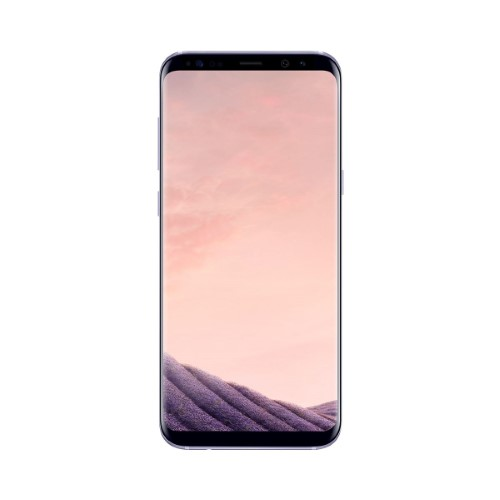
\includegraphics[width=5cm]{galaxy}};
\end{tikzpicture}
  \end{center}
\end{frame}
\begin{frame}
  \begin{center}
    \textbf{Text Generation: \\ Talk about Text (Translation / Summarization) }
  \end{center}
  \begin{center}
\begin{tikzpicture}
\node{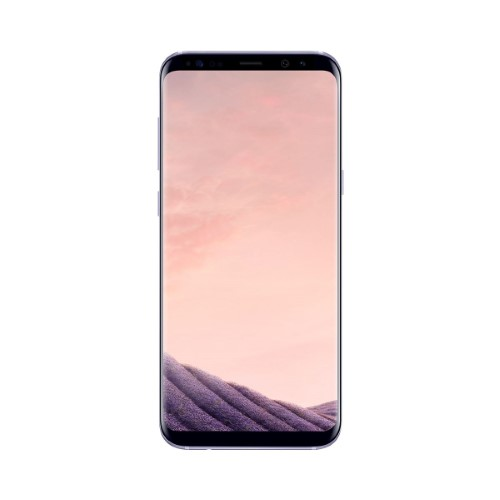
\includegraphics[width=5cm]{galaxy}};
\path<2>[draw] (0, 0) --  (2,0) ;

\node[inner sep=1pt, rounded corners, text width=15em, xshift=-4cm,]{\small

\vspace{0.5cm}
\tiny
mexico city , mexico -lrb- cnn -rrb- -- heavy rains and flooding have forced hundreds of thousands of people from homes in southern mexico 's state of tabasco over the past four days , with nearly as many trapped by the rising waters , state officials said thursday . officials say about 300,000 people are still trapped by the worst flooding in the region for 50 years . the grijalva river pushed over its banks through the state capital of villahermosa on thursday , forcing government workers to evacuate and leaving up to 80 percent of the city flooded , gov. andres granier 's office told cnn . about 700,000 people have seen their homes flooded , with about 300,000 of those still trapped there , granier 's office reported . one death had been blamed on the floods , which followed weeks of heavy rain in the largely swampy state . tabasco borders guatemala to the south and the gulf of mexico to the north . \ldots

};
\visible<2>{
\node [xshift=3.5cm, rectangle, draw,thick,fill=blue!0,text width=8em, rounded corners, inner sep =5pt, minimum height=1em]{\baselineskip=50pt \footnotesize tabasco and chiapas states hardest hit. authorities say 700,000 affected \ldots   \par};}
\end{tikzpicture}
  \end{center}
\end{frame}

\begin{frame}
  \begin{center}
    \textbf{Abstractive Sentence Summarization } \\
\small{ (Rush et al, 2015)}
  \end{center}
    \air

      Input (First Sentence)

  \begin{figure}
    \textit{\structure{Russian Defense Minister Ivanov}
      called \structure{Sunday} for \\ the creation of
      a joint front \structure{for combating} global terrorism. }
  \end{figure}

    Output (Title)
  \mair

  \begin{figure}
    \centering
    \textit{\alert{Russia} calls for joint
      front \alert{against} terrorism.}
  \end{figure}

\end{frame}



\begin{frame}
  \begin{center}
    \textbf{Text Generation: \\ Talk about Structured Data (Generation) }
  \end{center}
  \begin{center}
\begin{tikzpicture}
\node{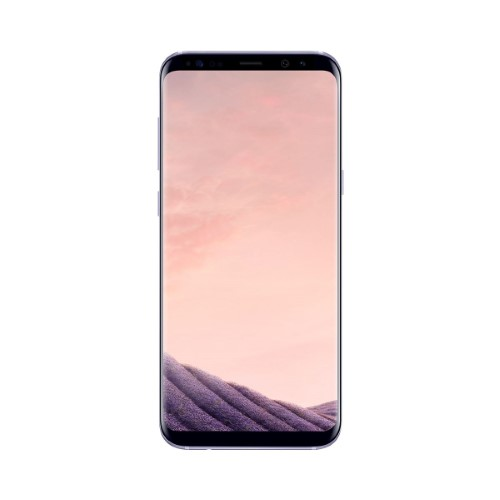
\includegraphics[width=5cm]{galaxy}};
\path<2>[draw] (0, 0) --  (2,0) ;
\node[inner sep=1pt, rounded corners, text width=15em, xshift=-4cm,]{\small
  \begin{center}
\vspace{0.5cm}
\footnotesize
\begin{tabular}{lcccccc}
\toprule
{} & W & L & PTS &  \ldots \\
TEAM &           &             &          &                      \\
\midrule
Heat   &        11 &          12 &      103 &     \ldots      \\
Hawks  &         7 &          15 &       95 &     \ldots      \\
\bottomrule

\vspace*{0.3cm}
\end{tabular}

% \begin{tabular}{lccccccccc}
% \toprule
% {} &  AS &    RB &   PT &  FG &  FGA & CITY  $\ldots$ \\
% PLAYER      &      &      &      &       &      &      &           \\
% \midrule
% Tyler Johnson    &    5 &    2 &  27 &    8 &   16 &     Miami \\
% Dwight Howard    &    11 &    17 &  23 &    9 &   11 &   Atlanta \\
% Paul Millsap     &    2 &    9 &  21 &    8 &   12 &   Atlanta \\
% Goran Dragic     &    4 &    2 &  21 &    8 &   17 &     Miami \\
% Wayne Ellington  &    2 &    3 &  19 &    7 &   15 &     Miami \\
% Dennis Schroder  &    7 &    4 &  17 &    8 &   15 &   Atlanta \\
% Rodney McGruder  &    5 &    5 &  11 &    3 &    8 &     Miami \\
% \ldots \\
% \bottomrule
% \end{tabular}

  \end{center}




};
 % \node [xshift=-3.5cm, rectangle, draw,thick,fill=blue!0,text width=8em, rounded corners, inner sep =5pt, minimum height=1em]{\baselineskip=50pt \footnotesize The Atlanta Hawks defeated the Miami Heat, 103 - 95, at Philips Arena on Wednesday. Atlanta  ... \par};
\visible<2>{\node[xshift=3.5cm, rectangle, draw,thick,fill=blue!0,text width=8em, rounded corners, inner sep =5pt, minimum height=1em]{\baselineskip=50pt \footnotesize The Atlanta Hawks defeated the Miami Heat, 103 - 95, at Philips Arena on Wednesday. Atlanta  ... \par};}
\end{tikzpicture}
  \end{center}
\end{frame}


\begin{frame}
% \centerline{\textbf{E2E Challenge 2018}}
% \air
\begin{center}
  
\includegraphics[width=0.5\textwidth]{e2e}
\end{center}
\begin{figure}[t]
\centering
\small
\begin{tabular}{@{}ll@{}}

\toprule
\bf MR        & \begin{tabular}[c]{@{}l@{}}name{[}The Golden Palace{]}, \\ eatType{[}coffee shop{]}, \\ food{[}Fast food{]}, \\ priceRange{[}cheap{]}, \\ customer rating{[}5 out of 5{]}, \\ area{[}riverside{]}\end{tabular}         \\ \midrule
\bf Reference & \begin{tabular}[c]{@{}l@{}}A coffee shop located on the riverside  called The Golden Palace,  \\ has a 5 out of 5 customer rating.  Its price range are fairly cheap  \\for its excellent Fast food.\end{tabular} \\ \bottomrule
\end{tabular}
\end{figure}
\end{frame}


\begin{frame}
  \begin{center}
    \textbf{ Text Generation: \\ Talk about the Environment (Multimodal) }
  \end{center}
  \begin{center}
\begin{tikzpicture}
\node{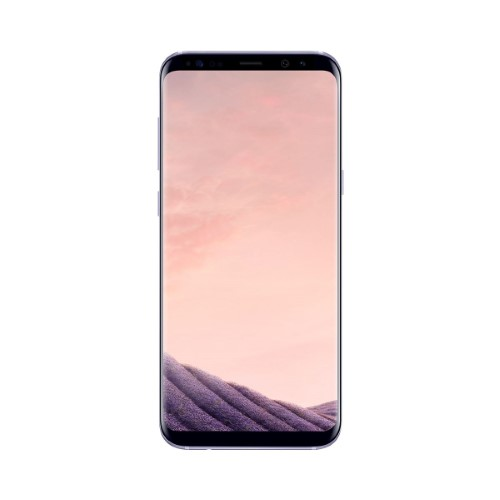
\includegraphics[width=5cm]{galaxy}};
\path<2>[draw] (0, 0) --  (2,0) ;
 \node [xshift=-4cm, rectangle, thick,fill=blue!0,text width=5cm, rounded corners, inner sep =5pt, minimum height=1em]{\baselineskip=50pt 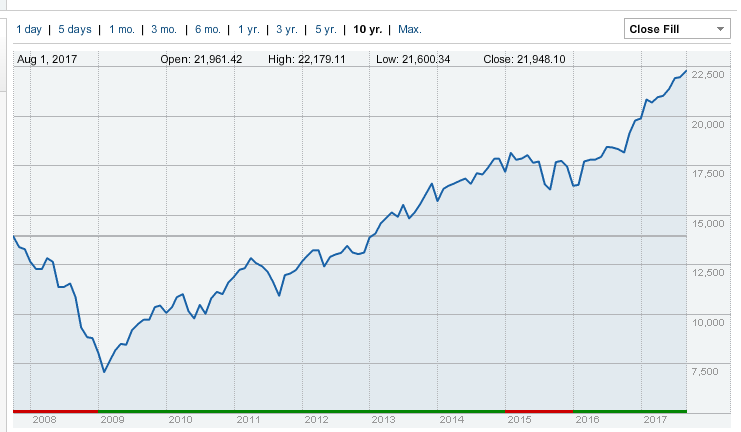
\includegraphics[width=5cm]{dowjones}};
\visible<2>{
\node [xshift=3.5cm, rectangle, draw,thick,fill=blue!0,text width=8em, rounded corners, inner sep =5pt, minimum height=1em]{\baselineskip=50pt \footnotesize Dow and S\&P 500 close out week at all-time highs ... \par};}
\end{tikzpicture}
  \end{center}
\end{frame}

\begin{frame}
  \centerline{\textbf{Image-to-Latex Dataset}}

  \centerline{\small (Deng et al, 2017)}
\air
\begin{center}
  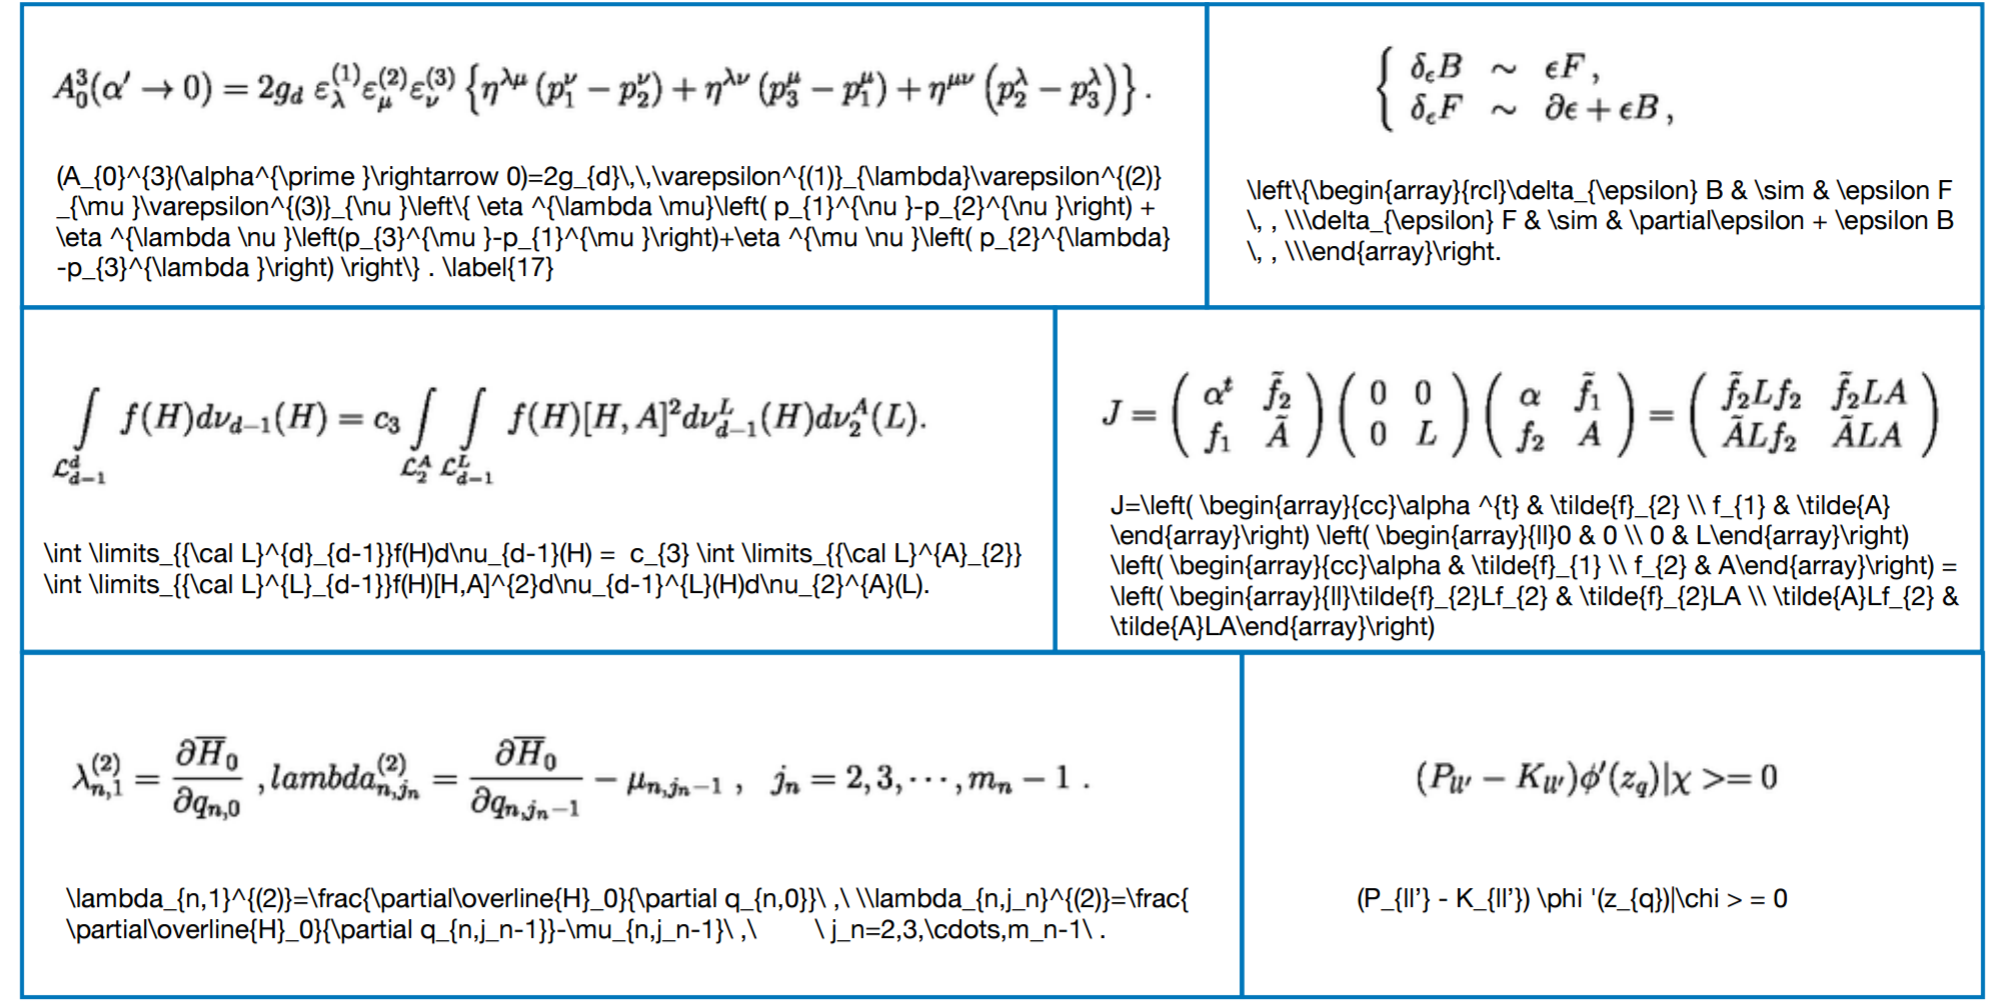
\includegraphics[height=0.6\textheight]{latex}
\end{center}
\end{frame}


\begin{frame}
  \centerline{\textbf{Image-to-Latex}}

  \centerline{\small (Deng et al, 2017)}
\air

  \begin{center}
    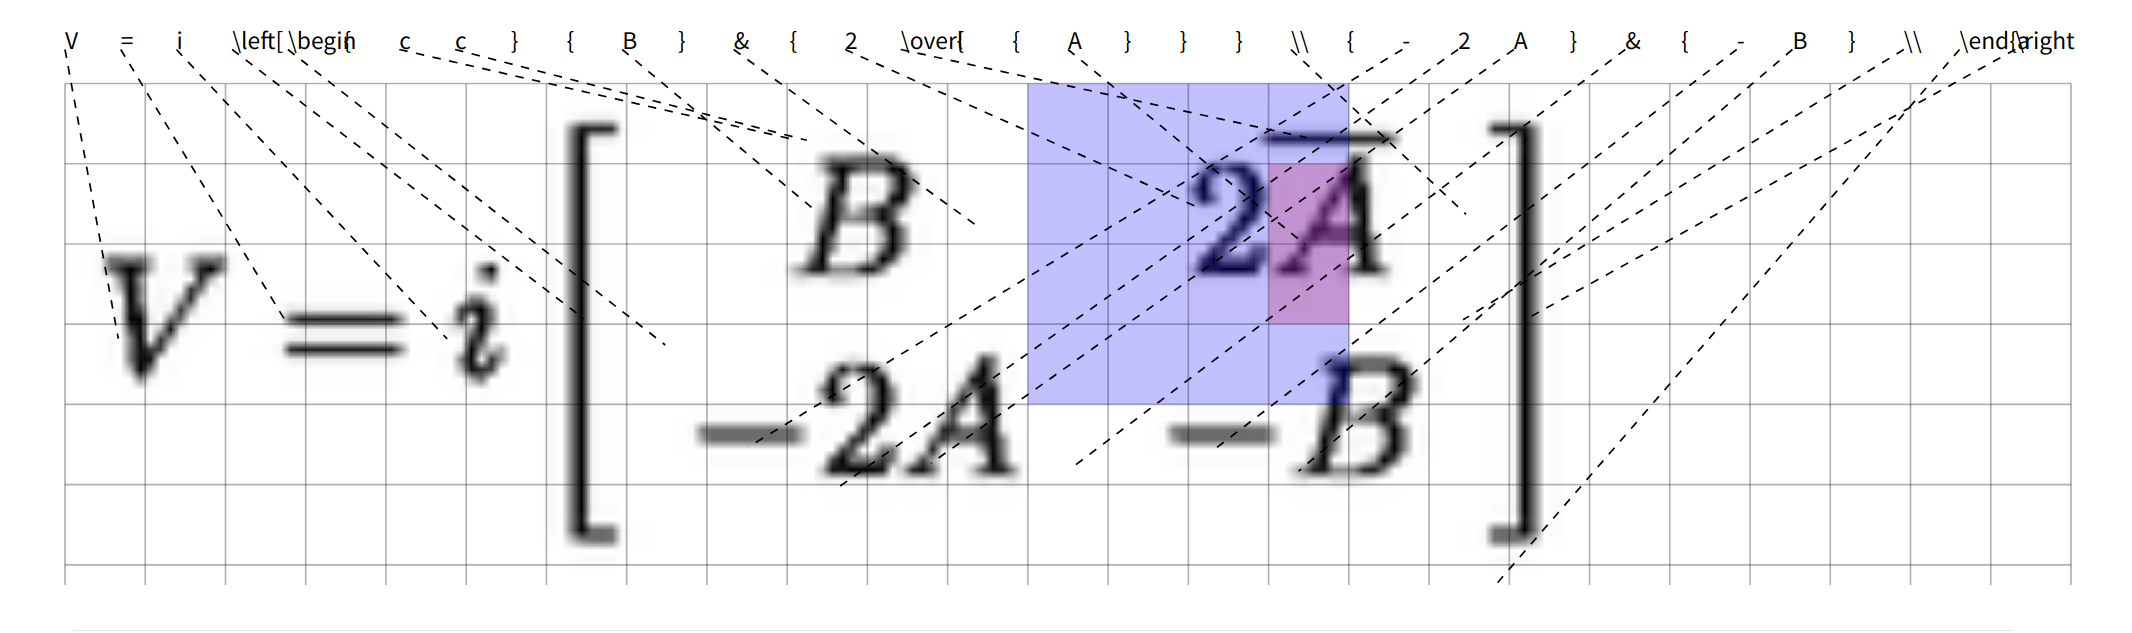
\includegraphics[width=0.9\linewidth]{ImageMark}
  \end{center}
\end{frame}



\begin{frame}
  \begin{center}
    \textbf{Seq2Seq+}  \air
  \end{center}
\center
\vspace{-5mm}
 \air
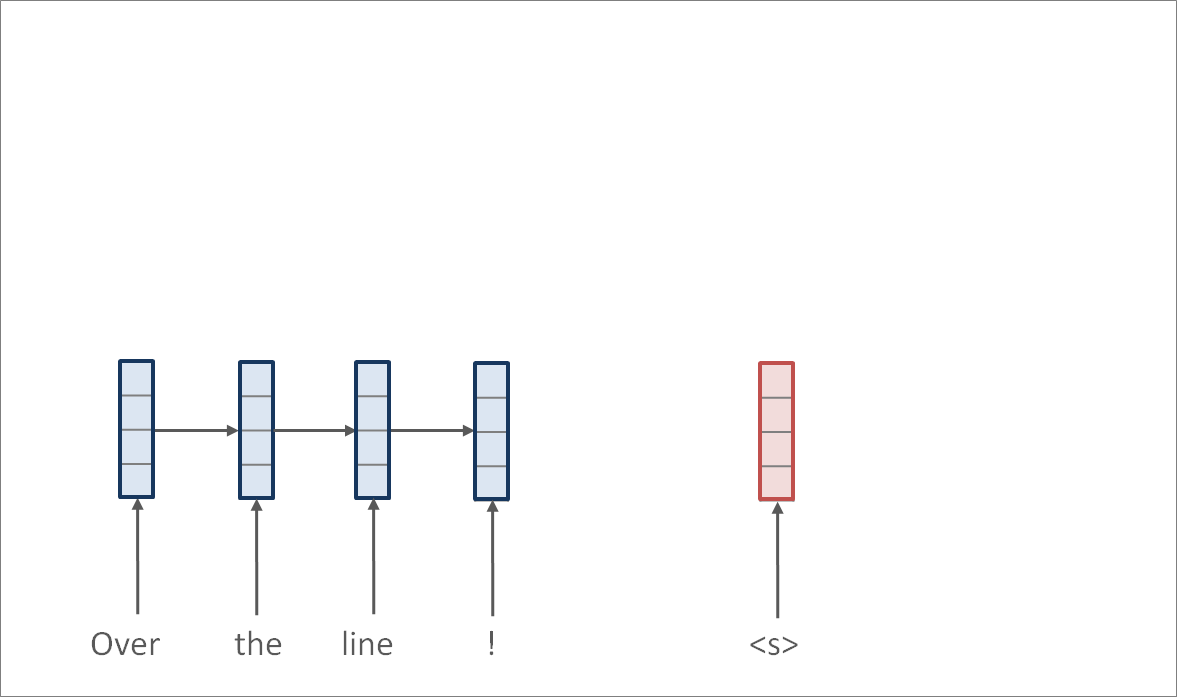
\includegraphics[scale=0.37]{nmt-attn1}
\end{frame}

\begin{frame}
  \begin{center}
    \textbf{Seq2Seq+} \air

  \end{center}
\center
\vspace{-5mm}
 \air
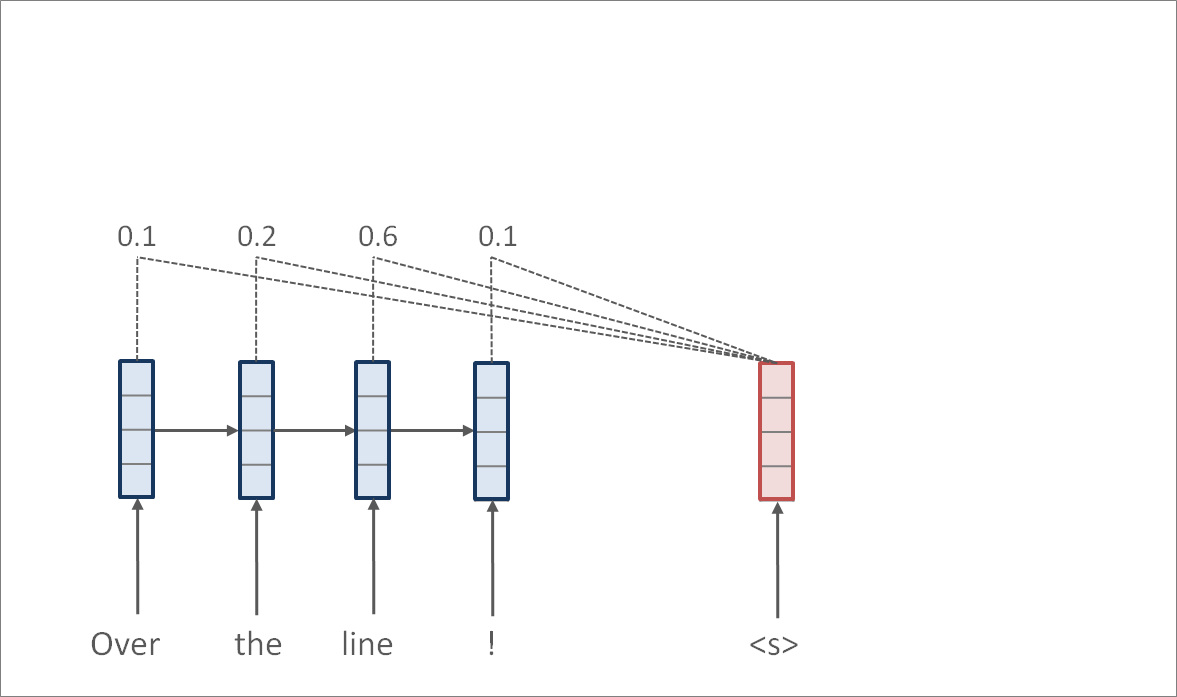
\includegraphics[scale=0.37]{nmt-attn2}
\end{frame}
\begin{frame}
  \begin{center}
    \textbf{Seq2Seq+} \air

  \end{center}
\center
\vspace{-5mm}
 \air
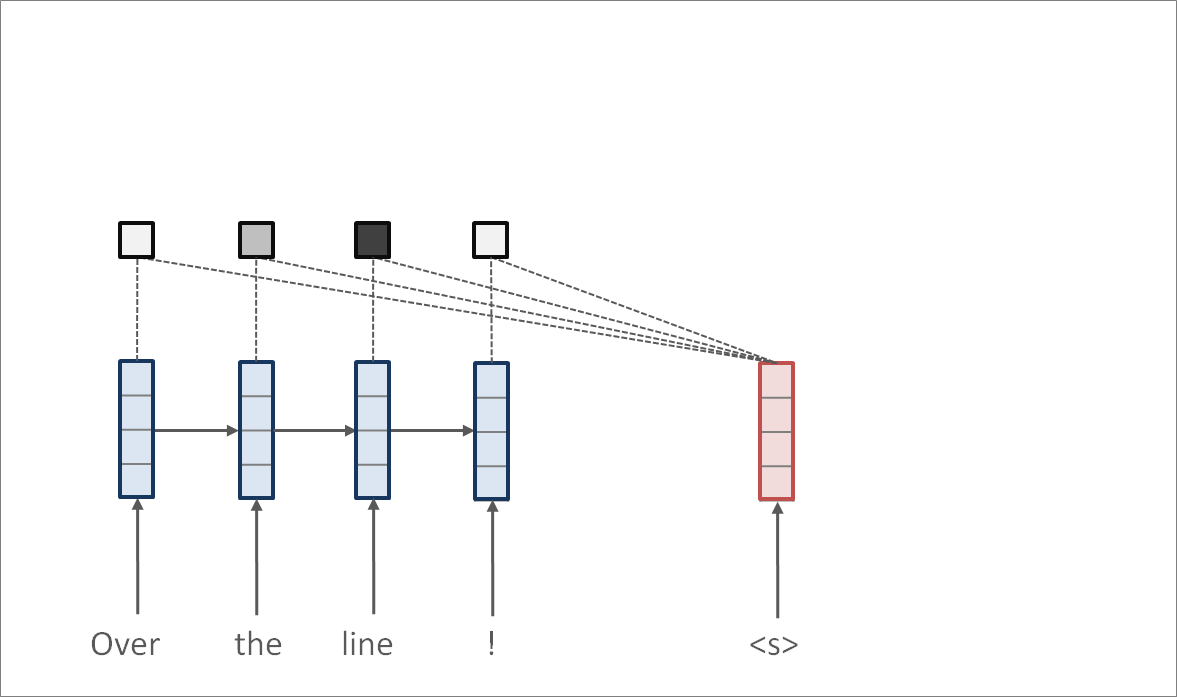
\includegraphics[scale=0.37]{nmt-attn3}
\end{frame}
\begin{frame}
  \begin{center}
    \textbf{Seq2Seq+} \air

  \end{center}
\center
\vspace{-5mm}
 \air
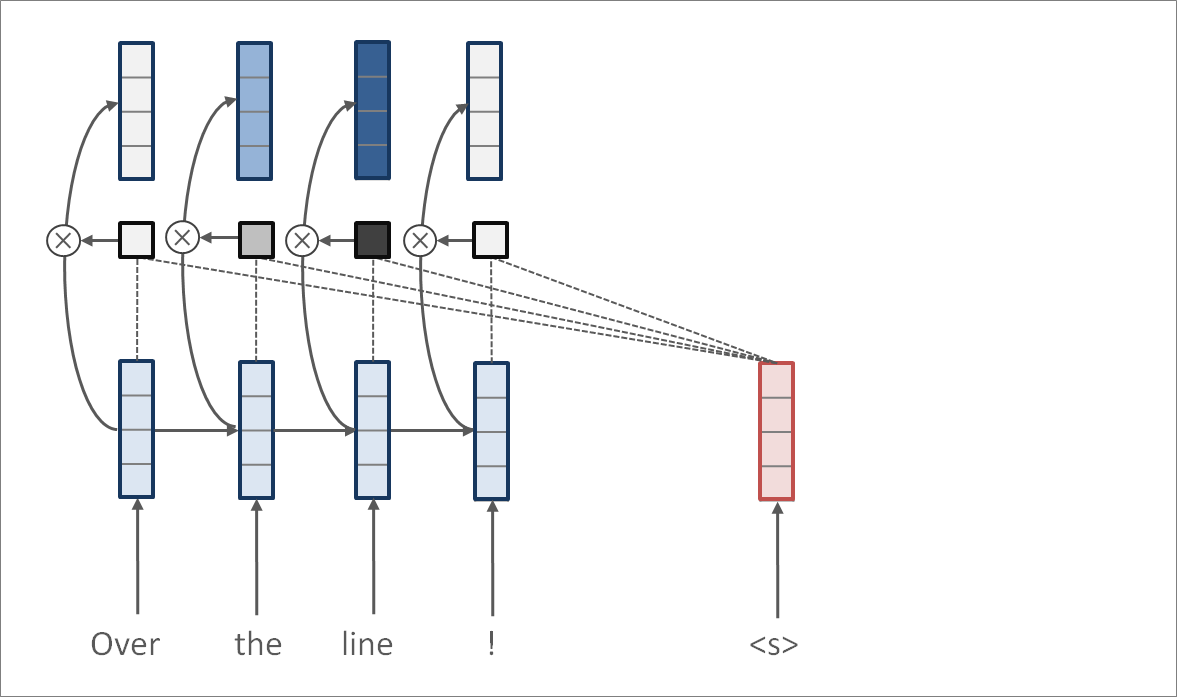
\includegraphics[scale=0.37]{nmt-attn4}
\end{frame}
\begin{frame}
  \begin{center}
    \textbf{Seq2Seq+} \air

  \end{center}
\center
\vspace{-5mm}
 \air
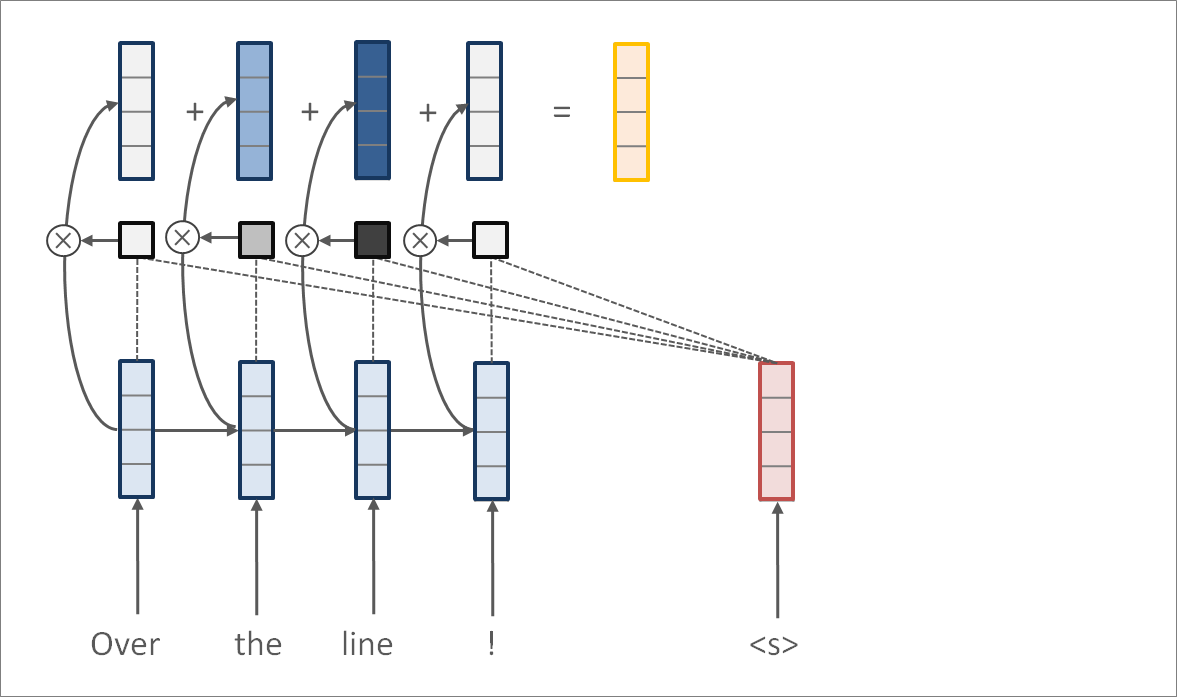
\includegraphics[scale=0.37]{nmt-attn5}
\end{frame}
\begin{frame}
  \begin{center}
    \textbf{Seq2Seq+} \air

  \end{center}
\center
\vspace{-5mm}
 \air
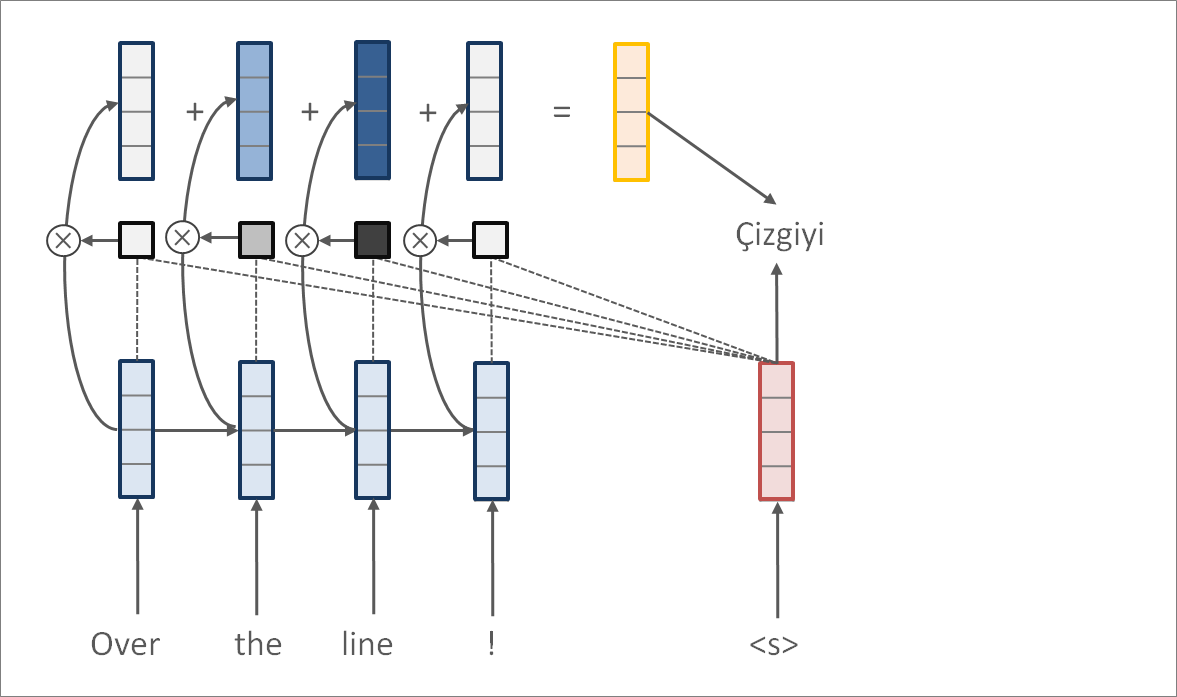
\includegraphics[scale=0.37]{nmt-attn6}
\end{frame}
\begin{frame}
  \begin{center}
    \textbf{Seq2Seq+} \air

  \end{center}
\center
\vspace{-5mm}
 \air
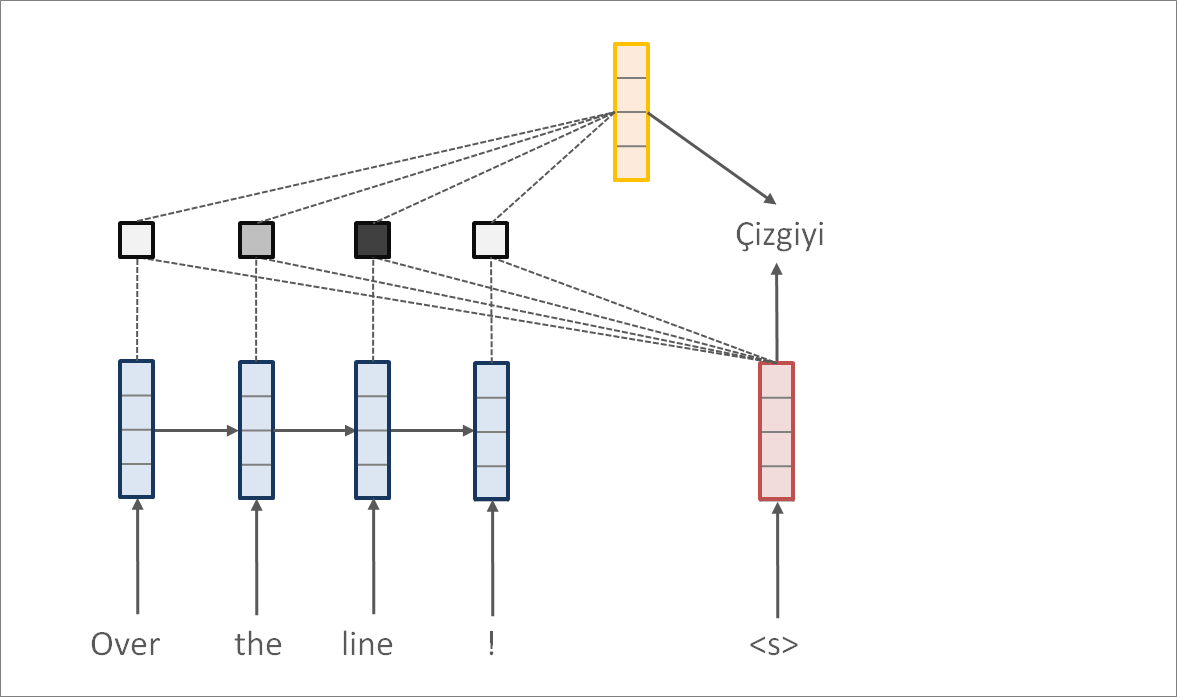
\includegraphics[scale=0.37]{nmt-attn7}
\end{frame}
\begin{frame}
  \begin{center}
    \textbf{Seq2Seq+} \air

  \end{center}
\center
\vspace{-5mm}
 \air
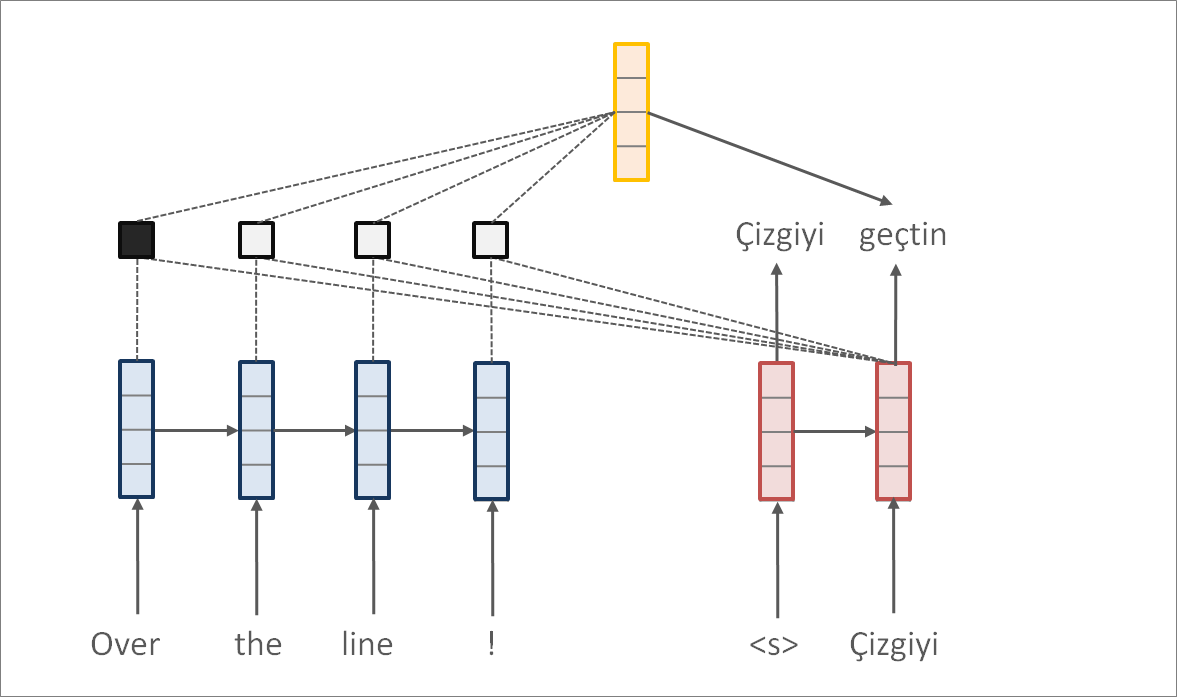
\includegraphics[scale=0.37]{nmt-attn8}
\end{frame}
\begin{frame}
  \begin{center}
    \textbf{Seq2Seq+} \air

  \end{center}
\center
\vspace{-5mm}
 \air
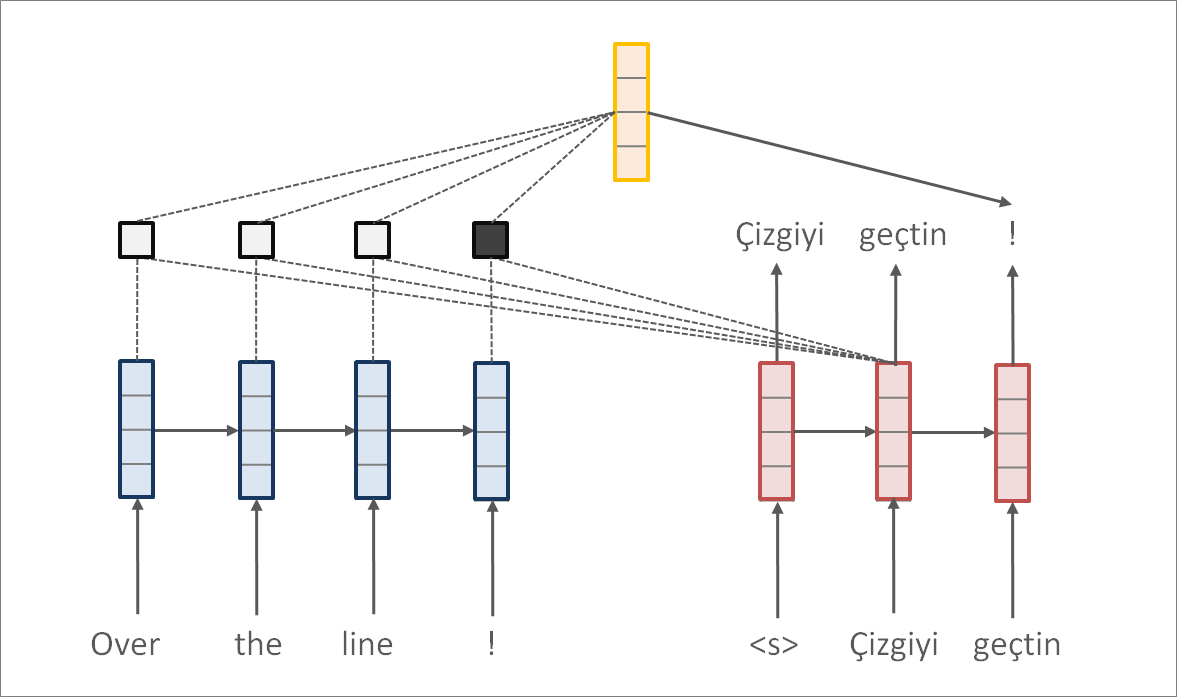
\includegraphics[scale=0.37]{nmt-attn9}
\end{frame}
\begin{frame}
  \begin{center}
    \textbf{Seq2Seq+} \air

  \end{center}
\center
\vspace{-5mm}
 \air
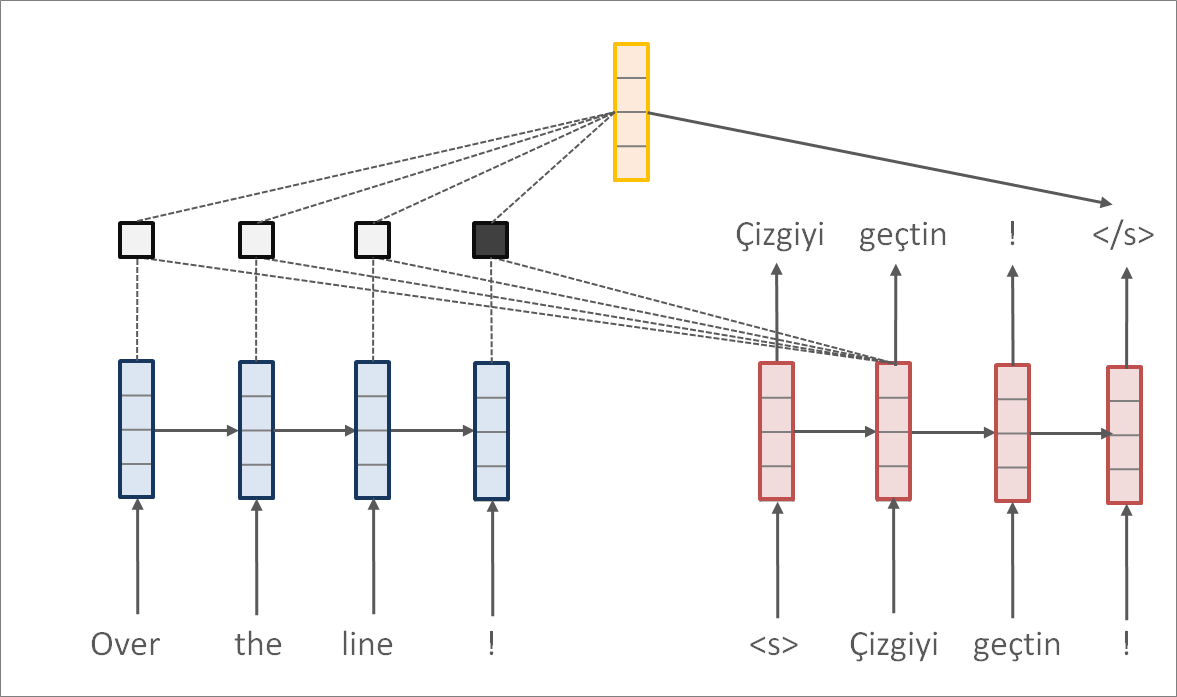
\includegraphics[scale=0.37]{nmt-attn10}
\end{frame}

% \begin{frame}
%   \centerline{\textbf{Seq2Seq+}}

%   \textcolor{blue}{Encoder} :
%   \[{\mathbf{h}^{x}_m \gets \RNN(\mathbf{h}^{x}_{m-1}, x_m)} \]


%   \textcolor{orange}{Attention}
%   \[\alpha \gets  \softmax(   [\mathbf{h}^{x}_1 ; \ldots; \mathbf{h}^{x}_M]^\top \mathbf{h}_{n} )\ \ \  {\mathbf{c}_n} \gets \sum_{m =1}^M \alpha_m \mathbf{h}_m^{x}  \]

%   \textcolor{red}{Decoder}:
%   \[{\mathbf{h}_n \gets \RNN(\mathbf{h}_{n-1}, w_n)} \]

%   Prediction
%   \[p(w_{n+1} | w_{1:n}, x_{1:M}) = \softmax( \mathbf{W} [\mathbf{h}_n, \mathbf{c}_n]) \]

% \end{frame}


% \begin{frame}
%   \begin{center}
%     \textbf{OpenNMT\\ {\small (Klein et al, 2017)}}

%   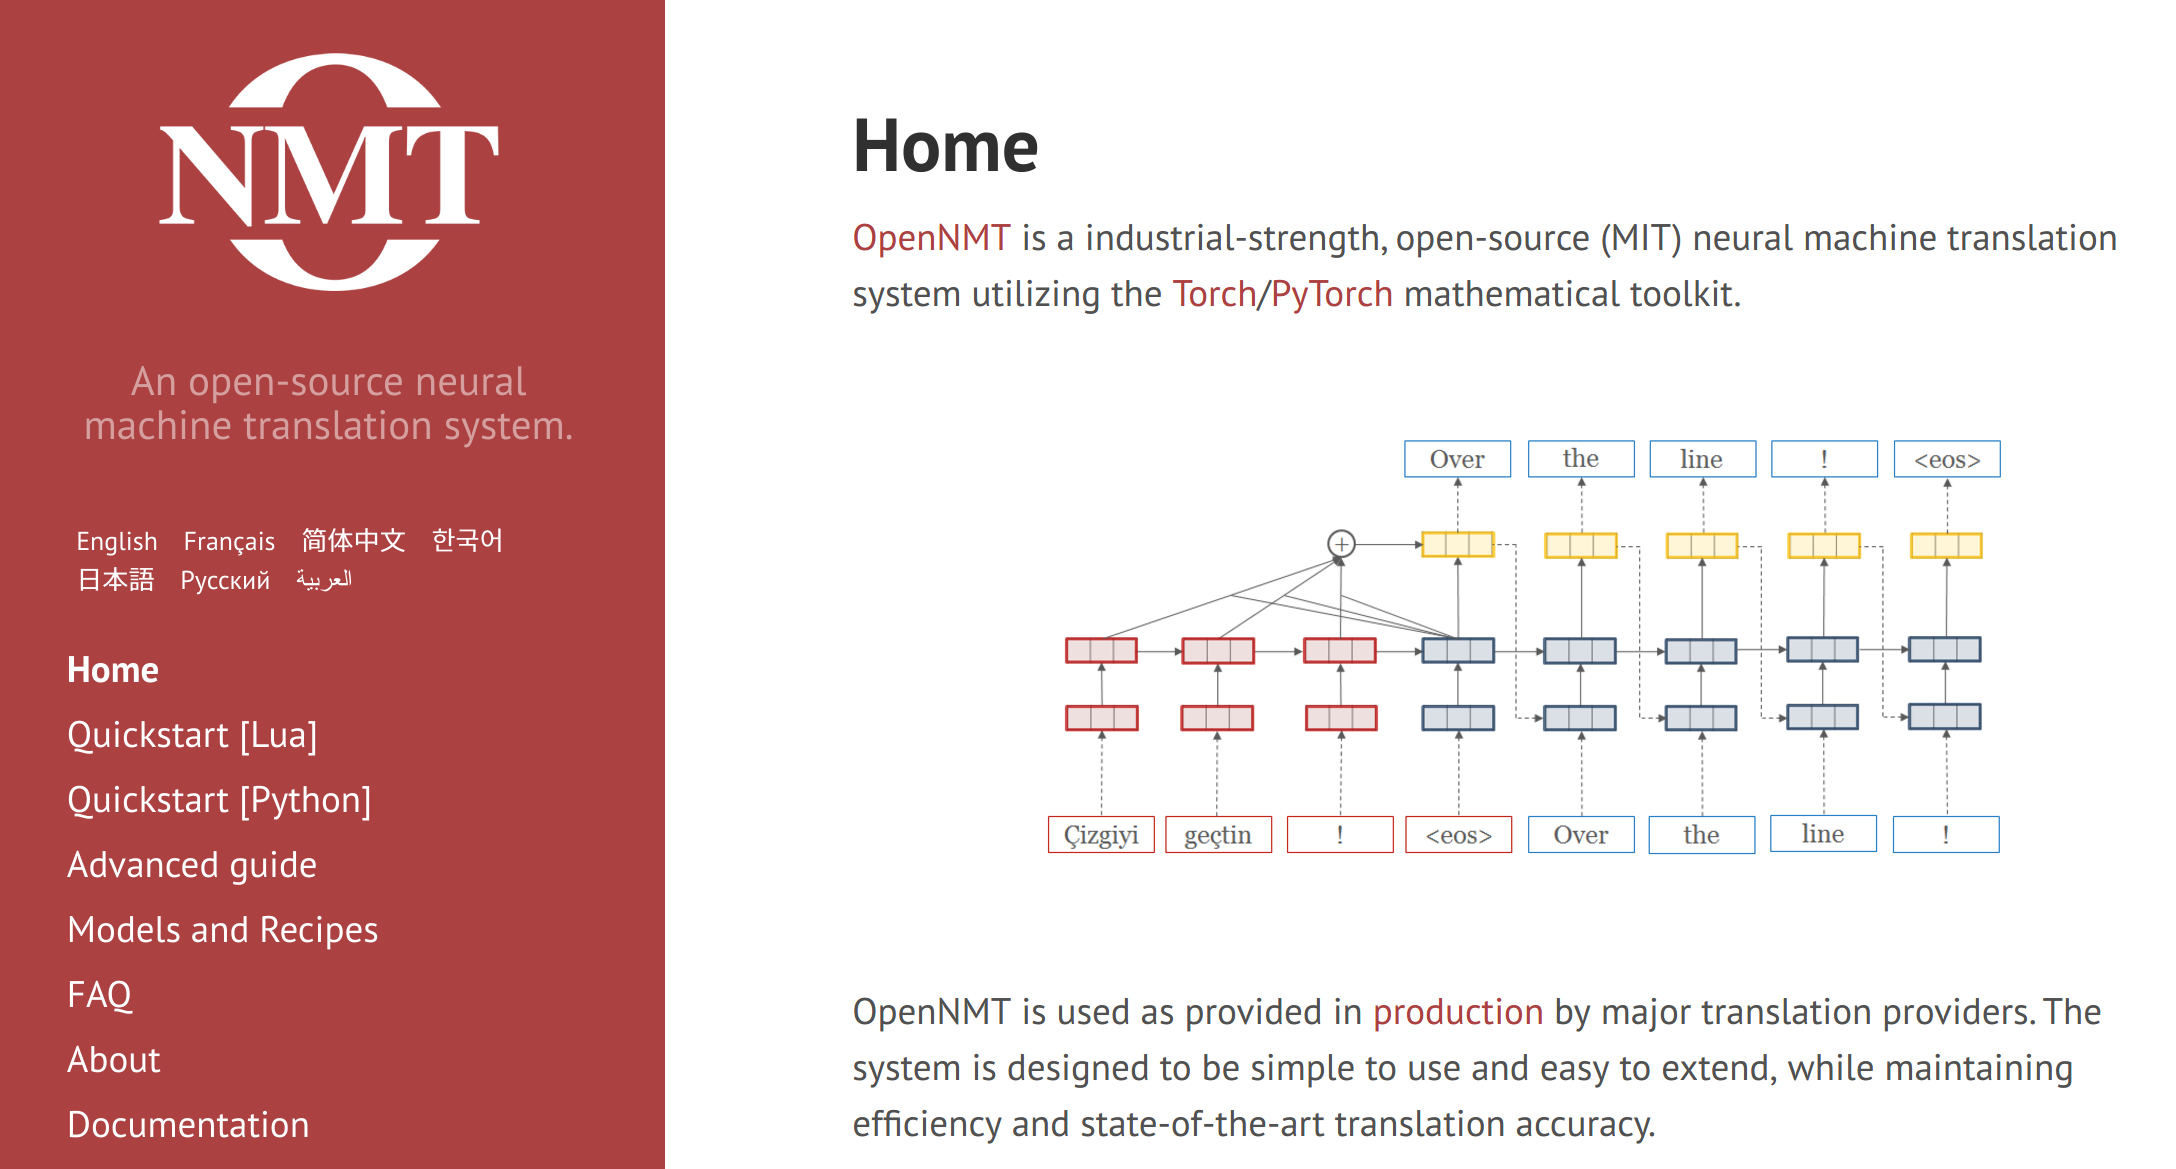
\includegraphics[width=10cm]{opennmt}
%   \end{center}

% \end{frame}

\begin{frame}
  \begin{center}
    \textbf{Seq2Seq-Vis \\ {\small (Strobelt et al, 2018)} }
  \end{center}

  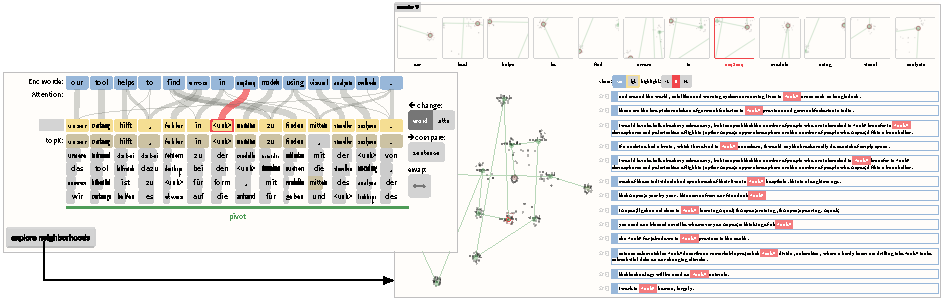
\includegraphics[width=\textwidth]{s2stease}
\end{frame}

\begin{frame}
  \begin{center}
    \textbf{Is generation solved by seq2seq? }
  \end{center}
\end{frame}

\begin{frame}
  \begin{center}
    \textbf{Challenges of Neural Generation  \\ {\small (Wiseman et al, 2017) } }
  \end{center}
  \begin{figure}
\centering
\scalebox{0.6}{
\begin{tikzpicture}
\node[draw, inner sep=10pt, rounded corners, text width=30em, xshift=-7.5cm,]{\small
  \begin{center}


\begin{tabular}{lcccccc}
\toprule
{} & WIN & LOSS & PTS & FG\_PCT & RB & AS \ldots \\
TEAM &           &             &          &             &          &          \\
\midrule
Heat      &        11 &          12 &      103 &          49 &       47 &       27 \\
Hawks     &         7 &          15 &       95 &          43 &       33 &       20 \\
\bottomrule
\end{tabular}
\vspace{0.5cm}

\begin{tabular}{lccccccccc}
\toprule
{} &  AS &    RB &   PT &  FG &  FGA & CITY  $\ldots$ \\
PLAYER      &      &      &      &       &      &      &           \\
\midrule
Tyler Johnson    &    5 &    2 &  27 &    8 &   16 &     Miami \\
Dwight Howard    &    11 &    17 &  23 &    9 &   11 &   Atlanta \\
Paul Millsap     &    2 &    9 &  21 &    8 &   12 &   Atlanta \\
Goran Dragic     &    4 &    2 &  21 &    8 &   17 &     Miami \\
Wayne Ellington  &    2 &    3 &  19 &    7 &   15 &     Miami \\
Dennis Schroder  &    7 &    4 &  17 &    8 &   15 &   Atlanta \\
Rodney McGruder  &    5 &    5 &  11 &    3 &    8 &     Miami \\
\ldots \\
\bottomrule
\end{tabular}

  \end{center}

};


\node [yshift=-4cm, rectangle, draw,thick,fill=blue!0,text width=30em, rounded corners, inner sep =10pt, minimum height=1em]{\baselineskip=100pt \large  The Atlanta Hawks defeated the Miami Heat, 103 - 95, at Philips Arena on Wednesday. Atlanta was in desperate need of a win and they were able to take care of a shorthanded Miami team here. Defense was key for the Hawks, as they held the Heat to 42 percent shooting and forced them to commit 16 turnovers. Atlanta also dominated in the paint, winning the rebounding battle, 47 - 34, and outscoring them in the paint 58 - 26. The Hawks shot 49 percent from the field and assisted on 27 of their 43 made baskets. This was a near wire-to-wire win for the Hawks, as Miami held just one lead in the first five minutes. Miami ( 7 - 15 ) are as beat-up as anyone right now and it's taking a toll on the heavily used starters. Hassan Whiteside really struggled in this game, as he amassed eight points, 12 rebounds and one blocks on 4 - of - 12 shooting ... \par};
\end{tikzpicture}
}
\caption{\small Document generation example. Left, a source consisting of structured data, in this case statistics from a basketball game. Right, a target document utilizing a select subset of records from the data,
  expressed in an often complex and expressive manner. This example is an excerpt from the case-study data set, which include
  628 records in total and a longer target document. }
\label{fig:samplesummary}
\end{figure}


\end{frame}

\begin{frame}
  \begin{center}
    \textbf{Challenges of Neural Generation  \\ {\small (Wiseman et al, 2017) } }
  \end{center}

  \begin{figure}
\centering
\scalebox{0.9}{\begin{tikzpicture}
    \node[text width=12cm, draw, rounded corners, inner sep=10pt]{\small
  The \textcolor<2>{blue}{Utah Jazz} ( \textcolor<2>{blue}{38} - \textcolor<2>{red}{26} ) \textcolor<2>{red}{defeated} the \textcolor<2>{blue}{Houston Rockets} ( \textcolor<2>{red}{38} - \textcolor<2>{blue}{26} ) \textcolor<2>{blue}{117 - 91} on Wednesday at \textcolor<2>{blue}{Energy Solutions Arena in Salt Lake City} . The \textcolor<2>{blue}{Jazz} got out to a quick start in this one , out - scoring the \textcolor<2>{blue}{Rockets} \textcolor<2>{blue}{31} - \textcolor<2>{red}{15} in the first quarter alone . Along with the quick start , the \textcolor<2>{blue}{Rockets} were the superior shooters in this game , going \textcolor<2>{blue}{54 percent from the field} and \textcolor<2>{blue}{43 percent from the three - point line} , while the \textcolor<2>{blue}{Jazz} went \textcolor<2>{blue}{38} percent from the floor and a meager \textcolor<2>{blue}{19} percent from deep . The \textcolor<2>{blue}{Rockets} were able to out - rebound the \textcolor<2>{red}{Rockets} \textcolor<2>{blue}{49} - \textcolor<2>{red}{49} , giving them just enough of an advantage to secure the victory in front of their \textcolor<2>{red}{home crowd} . The \textcolor<2>{blue}{Jazz} were led by the duo of \textcolor<2>{blue}{Derrick Favors} and \textcolor<2>{red}{James Harden} . Favors went \textcolor<2>{blue}{2 - for - 6} from the field and \textcolor<2>{blue}{0 - for - 1} from the three - point line to score a \textcolor<2>{red}{game - high} of \textcolor<2>{red}{15 points} , while also adding \textcolor<2>{blue}{four rebounds} and \textcolor<2>{red}{four assists} ....};
  \end{tikzpicture}}
\end{figure}
\begin{center}
\end{center}
\end{frame}

\begin{frame}
  \centerline{\textbf{Quantitative Evaluation / RotoWire}}
  \begin{table}
    \small
    \centering
    \begin{tabular}{lcccccc}
      \toprule
       & \multicolumn{5}{c}{} \\
       & \multicolumn{2}{c}{Relations}  & \multicolumn{2}{c}{Content} & Ordering \\
      Model & P\% & \# & P\% & R\% & DLD\%  & BLEU\\
      \midrule
      % &Gold                     & 91.77 & 12.84 & 100   & 100  & 100   \\
      Template                 & \textbf{99.35} & 49.7  & \textbf{45.17} & 24.85 & \textbf{12.2} & 6.87    \\
      \midrule
      Seq2Seq+Copy        &   71.07 & 12.61 & 21.90 & 27.27 & 8.70 & \textbf{14.46}\\
      \bottomrule
    \end{tabular}
  \end{table}
\end{frame}




\section{Controlling Generation}

\begin{frame}
  \begin{center}
    \textbf{ What is Missing for  Generation? }
  \end{center}

    \textit{Building Natural Language Generation Systems} (Reiter and Dale, 1999)

 \begin{center}
    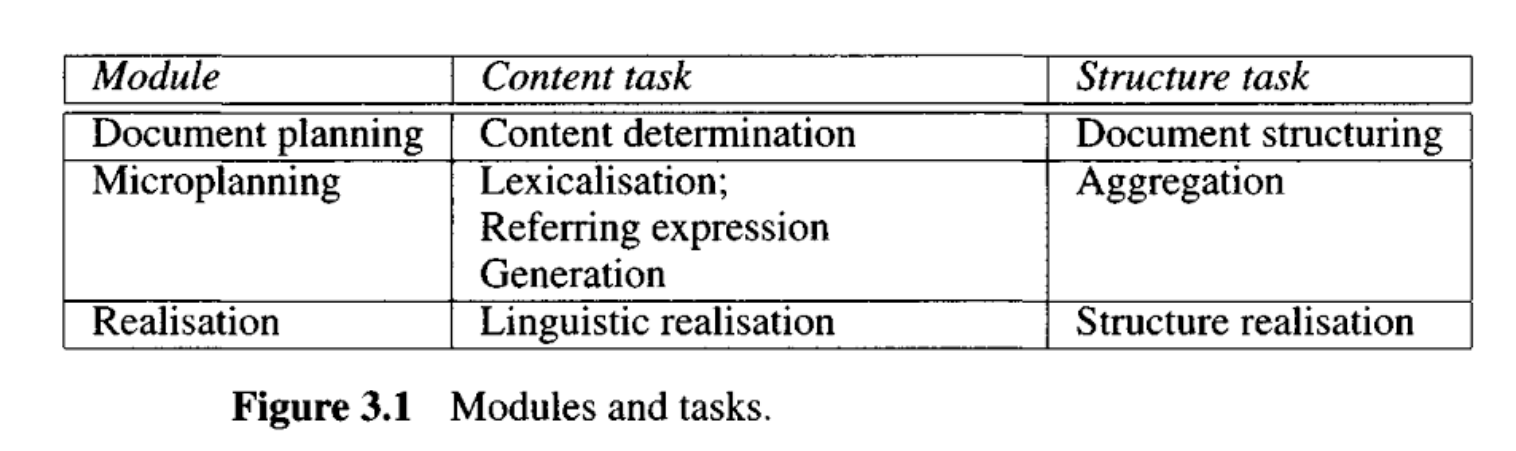
\includegraphics[width =12cm]{datadoc}
  \end{center}

\end{frame}


% \begin{frame}
%   \begin{center}
%     \structure{The Modern Text Generation Challenge: \\ Make Some Conversation (Chatbots)}
%   \end{center}
%   \begin{center}
% \begin{tikzpicture}
% \node{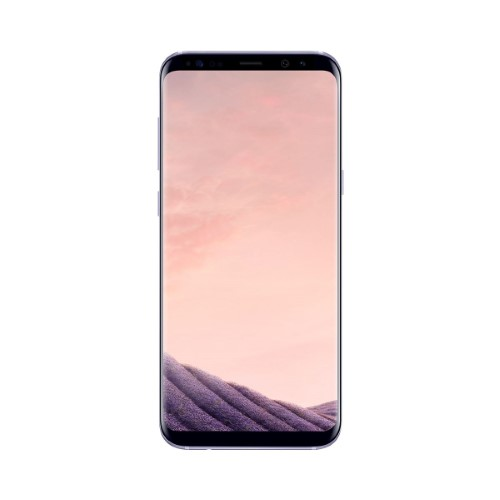
\includegraphics[width=5cm]{galaxy}};
% \path[draw] (0, 0) --  (2,0) ;
% \node [xshift=3.5cm, rectangle, draw,thick,fill=blue!0,text width=8em, rounded corners, inner sep =5pt, minimum height=1em]{\baselineskip=50pt \footnotesize Hi there Joe, have a good day today!  \par};
% \end{tikzpicture}
%   \end{center}
% \end{frame}



% \begin{frame}
%   \begin{center}
%     \textbf{Are these problems just Seq2Seq?}

%     \begin{itemize}
%     \item Certainly the key aspect of their success.
%       \air

%     \item However there has slowly tentative steps towards problem
%       specific modeling.
%     \end{itemize}
%   \end{center}
% \end{frame}


% \begin{frame}
%   \begin{center}
%     \textbf{Case Study: Seq2Seq+Copy}

%     \small{(Gu et al, 2016) (Gulcehre et al, 2016) ...}
%   \end{center}
%   \textcolor{blue}{Encoder} :
%   \[{\mathbf{h}^{x}_m \gets \RNN(\mathbf{h}^{x}_{m-1}, x_m)} \]


%   \textcolor{orange}{Attention}
%   \[\alpha \gets  \softmax(   [\mathbf{h}^{x}_1 ; \ldots; \mathbf{h}^{x}_M]^\top \mathbf{h}_{n} )\ \ \ {\mathbf{c}_n} \gets \sum_{m =1}^M \alpha_m \mathbf{h}_m^{x}  \]

%   \textcolor{red}{Decoder}:
%   \[{\mathbf{h}_n \gets \RNN(\mathbf{h}_{n-1}, w_n)} \]

%   Prediction
%   \begin{eqnarray*}
%   p(w_{n+1} | w_{1:n}, x_{1:M}) = & p(z = 1 |  w_{1:n}, x_{1:M}) \times \softmax( \mathbf{W} [\mathbf{h}_n, \mathbf{c}_n])   \\+ &\displaystyle p(z=0 | w_{1:n}, x_{1:M}) \times \sum_{m: x_m = w_{n+1}} \alpha_m
%   \end{eqnarray*}
% \end{frame}

% \begin{frame}
% \begin{center}
%     \textbf{Copy is Critical For Summarization }
%     \\
%     \small{(See et al. 2017)}
%       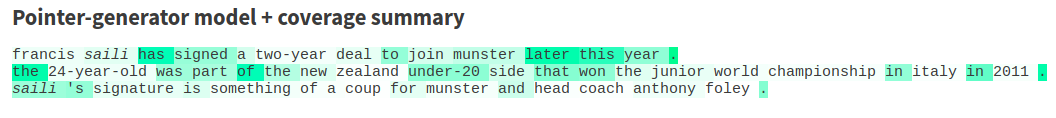
\includegraphics[width=15cm]{seeblog}
% \pause

%       \textbf{Bottom-Up Summarization}

%  (Gehrmann et al, 2018)


%  \begin{itemize}
%  \item Shows that controlling copying alone produces state-of-the-art
%    results.
%  \end{itemize}
% \end{center}
% \end{frame}




% \section{Latent-Variable Generation}




\begin{frame}
\begin{center}
    \textbf{Research Direction: \\
      Deep Discrete Latent-Variable Models for NLP }
  \end{center}
  Goal: Expose controls as \textit{discrete} latent variables.


\begin{align*}
p(y, z \param \theta).
\end{align*}

\begin{itemize}
    \item $y$ is our observed data
    \item $z$ is a collection of problem-specific latent variables
    \item $\theta$ are the deterministic, neural network parameters.
\end{itemize}

% \begin{itemize}
%     \item Data consists of $N$ i.i.d samples,
% \end{itemize}

%                 \[ p(x^{(1:N)}, z^{(1:N)} \param \theta ) = \prod_{n=1}^N p(x^{(n)} \given z^{(n)}; \theta) p(z^{(n)};\theta). \]

\end{frame}

\begin{frame}
\thetitle{Example Model: Mixture of RNNs}

Generative process:
\begin{enumerate}
\item Draw cluster $z \in \{1, \ldots, K\}$ from a Categorical.
\item Draw words $y_{1:T}$ from RNNLM with parameters $\pi_z$.
\end{enumerate}
\[p(y, z \param \theta)
       = \mu_{z} \times   \RNNLM(y_{1:T} \param \pi_z) \]
% \[p(x, z \param \theta)
%       = \mu_{z} \times  \prod_{t=1}^T \softmax(\RNN(\boldh_{t-1}, x_t\param \pi_z))\]
\begin{center}

\begin{tikzpicture}
  %\tikz{
% nodes
\node (dots) {$\ldots$};%
 \node[obs, left=1cm of dots] (x1) {$y_1^{(n)}$};%
 \node[obs, right=1cm of dots] (xT) {$y_T^{(n)}$};%
 \node[latent, above=of dots] (z) {$z^{(n)}$}; %
 \node[const, above=(0.5cm) of z] (mu) {$\mu$};
 \node[const, below left=0.3cm and 0.8cm of x1] (pi) {$\pi$};

% plate
 \plate {plate1} {(dots)(x1)(xT)(z)} {$N$}; %
% edges
 \edge {z} {dots};
 \edge {z} {x1};
 \edge {z} {xT};
 \edge {mu} {z};
 \edge {pi.east} {x1,xT.south};
 \edge {x1} {dots};
 %\edge[bend left] {x1.south} {xT.south};
  \edge {dots} {xT};

 \draw[->]
 (x1) edge[bend right=10] node [right] {} (xT);
 %}
 \end{tikzpicture}
 %}
\end{center}
%\begin{align*}
%\boldh_{z,t} &= \tanh(\mathbf{W}_z \bolde_t +\mathbf{U}_z\boldh_{z,t-1}  + \boldb_{z}) \nonumber \\
%p(x_{t} \given x_{<t} , z) &= \softmax(\mathbf{V} \boldh_{z,t-1} + \boldc)_{x_{t}} \nonumber \\
%p(x_1, \ldots, x_T \given z) &= \prod_{t=1}^{T} p(x_{t} \given x_{<t} , z)
%\end{align*}


\end{frame}


% begin{frame}
% \begin{center}
%     \textbf{ Latent-Variable Model Basics }
%   \end{center}


% \begin{align*}
% p(x, z \param \theta).
% \end{align*}

% \pause
% \begin{itemize}
%     \item $x$ is our observed data
%     \item $z$ is a collection of latent variables
%     \item $\theta$ are the deterministic parameters of the model, such as the neural network parameters
% \end{itemize}

% \pause

% \begin{itemize}
%     \item Data consists of $N$ i.i.d samples,
% \end{itemize}


%                 \[ p(x^{(1:N)}, z^{(1:N)} \param \theta ) = \prod_{n=1}^N p(x^{(n)} \given z^{(n)}; \theta) p(z^{(n)};\theta). \]
% \end{frame}

\begin{frame}\thetitle{Main Requirement: Posterior Inference}
    For models $p(y, z \param \theta)$, we'll be interested in the \textit{posterior} over latent variables $z$:

    \begin{align*}
        p(z \given y \param \theta) = \frac{\displaystyle p(y, z \param \theta)}{\displaystyle p(y \param \theta)} = \frac{\displaystyle p(y\given z \param  \theta) p(z \param  \theta)}{\displaystyle \sum_{z'} p(y \given z'\param  \theta) p(z'\param  \theta) }.
    \end{align*}

    \air



% \item Intuition: if I know likely $z^{(n)}$ for $x^{(n)}$, I can learn by maximizing $p(x^{(n)} \given z^{(n)} \param \theta)$.
        % \begin{itemize}
        %     \item Intuition: if I know likely $z^{(n)}$ for $x^{(n)}$, I can learn by maximizing $p(x^{(n)} \given z^{(n)} \param \theta)$.
        % \end{itemize}


    How?

    \begin{itemize}
    \item Sum out over all discrete choices (e.g. run $K$ RNNs).
    \item Variational inference based methods.
    \end{itemize}
    Why?
    \begin{itemize}
      \item Required for training
      \item Latent $z$ gives separation of data.
    \end{itemize}
\end{frame}


\begin{frame}
  \begin{center}
    \textbf{ In Applications: Copy-Attention \\
      \small{(Gu et al, 2016) (Gulcehre et al, 2016)}}
  \end{center}

Let $z$ be a binary latent variable.
\air
\begin{itemize}
\item If $z = 1$, let the model generate a new word.
\item If $z = 0$, let the model copy a word from the source based on attention.
\end{itemize}

Inference:
\begin{center}


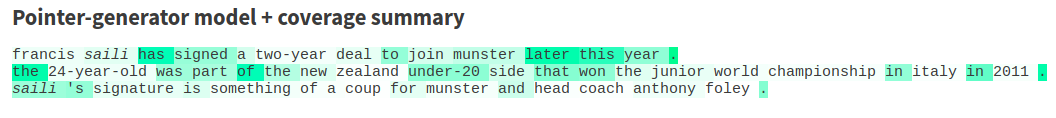
\includegraphics[width=15cm]{seeblog}

\centerline{\small (See et al, 2017)}
\end{center}
\end{frame}



% \begin{frame}
%   \begin{center}
%     \textbf{ Latent Variable Models for Generation}
%   \end{center}

%   \begin{itemize}
%   \item Can we develop other discrete latent-variable models for generation?
%     \air
%   \item Perhaps each important aspect of generation can be built-in directly.
%     \air
%   \item Goals:
%     \begin{itemize}
%     \item Model Control
%     \item Model Debugging
%     \item Model Uncertainty
%     \end{itemize}
%   \end{itemize}
% \end{frame}





\begin{frame}
  \begin{center}
    \textbf{Today: Learning Neural Templates}
  \end{center}

  \begin{center}
    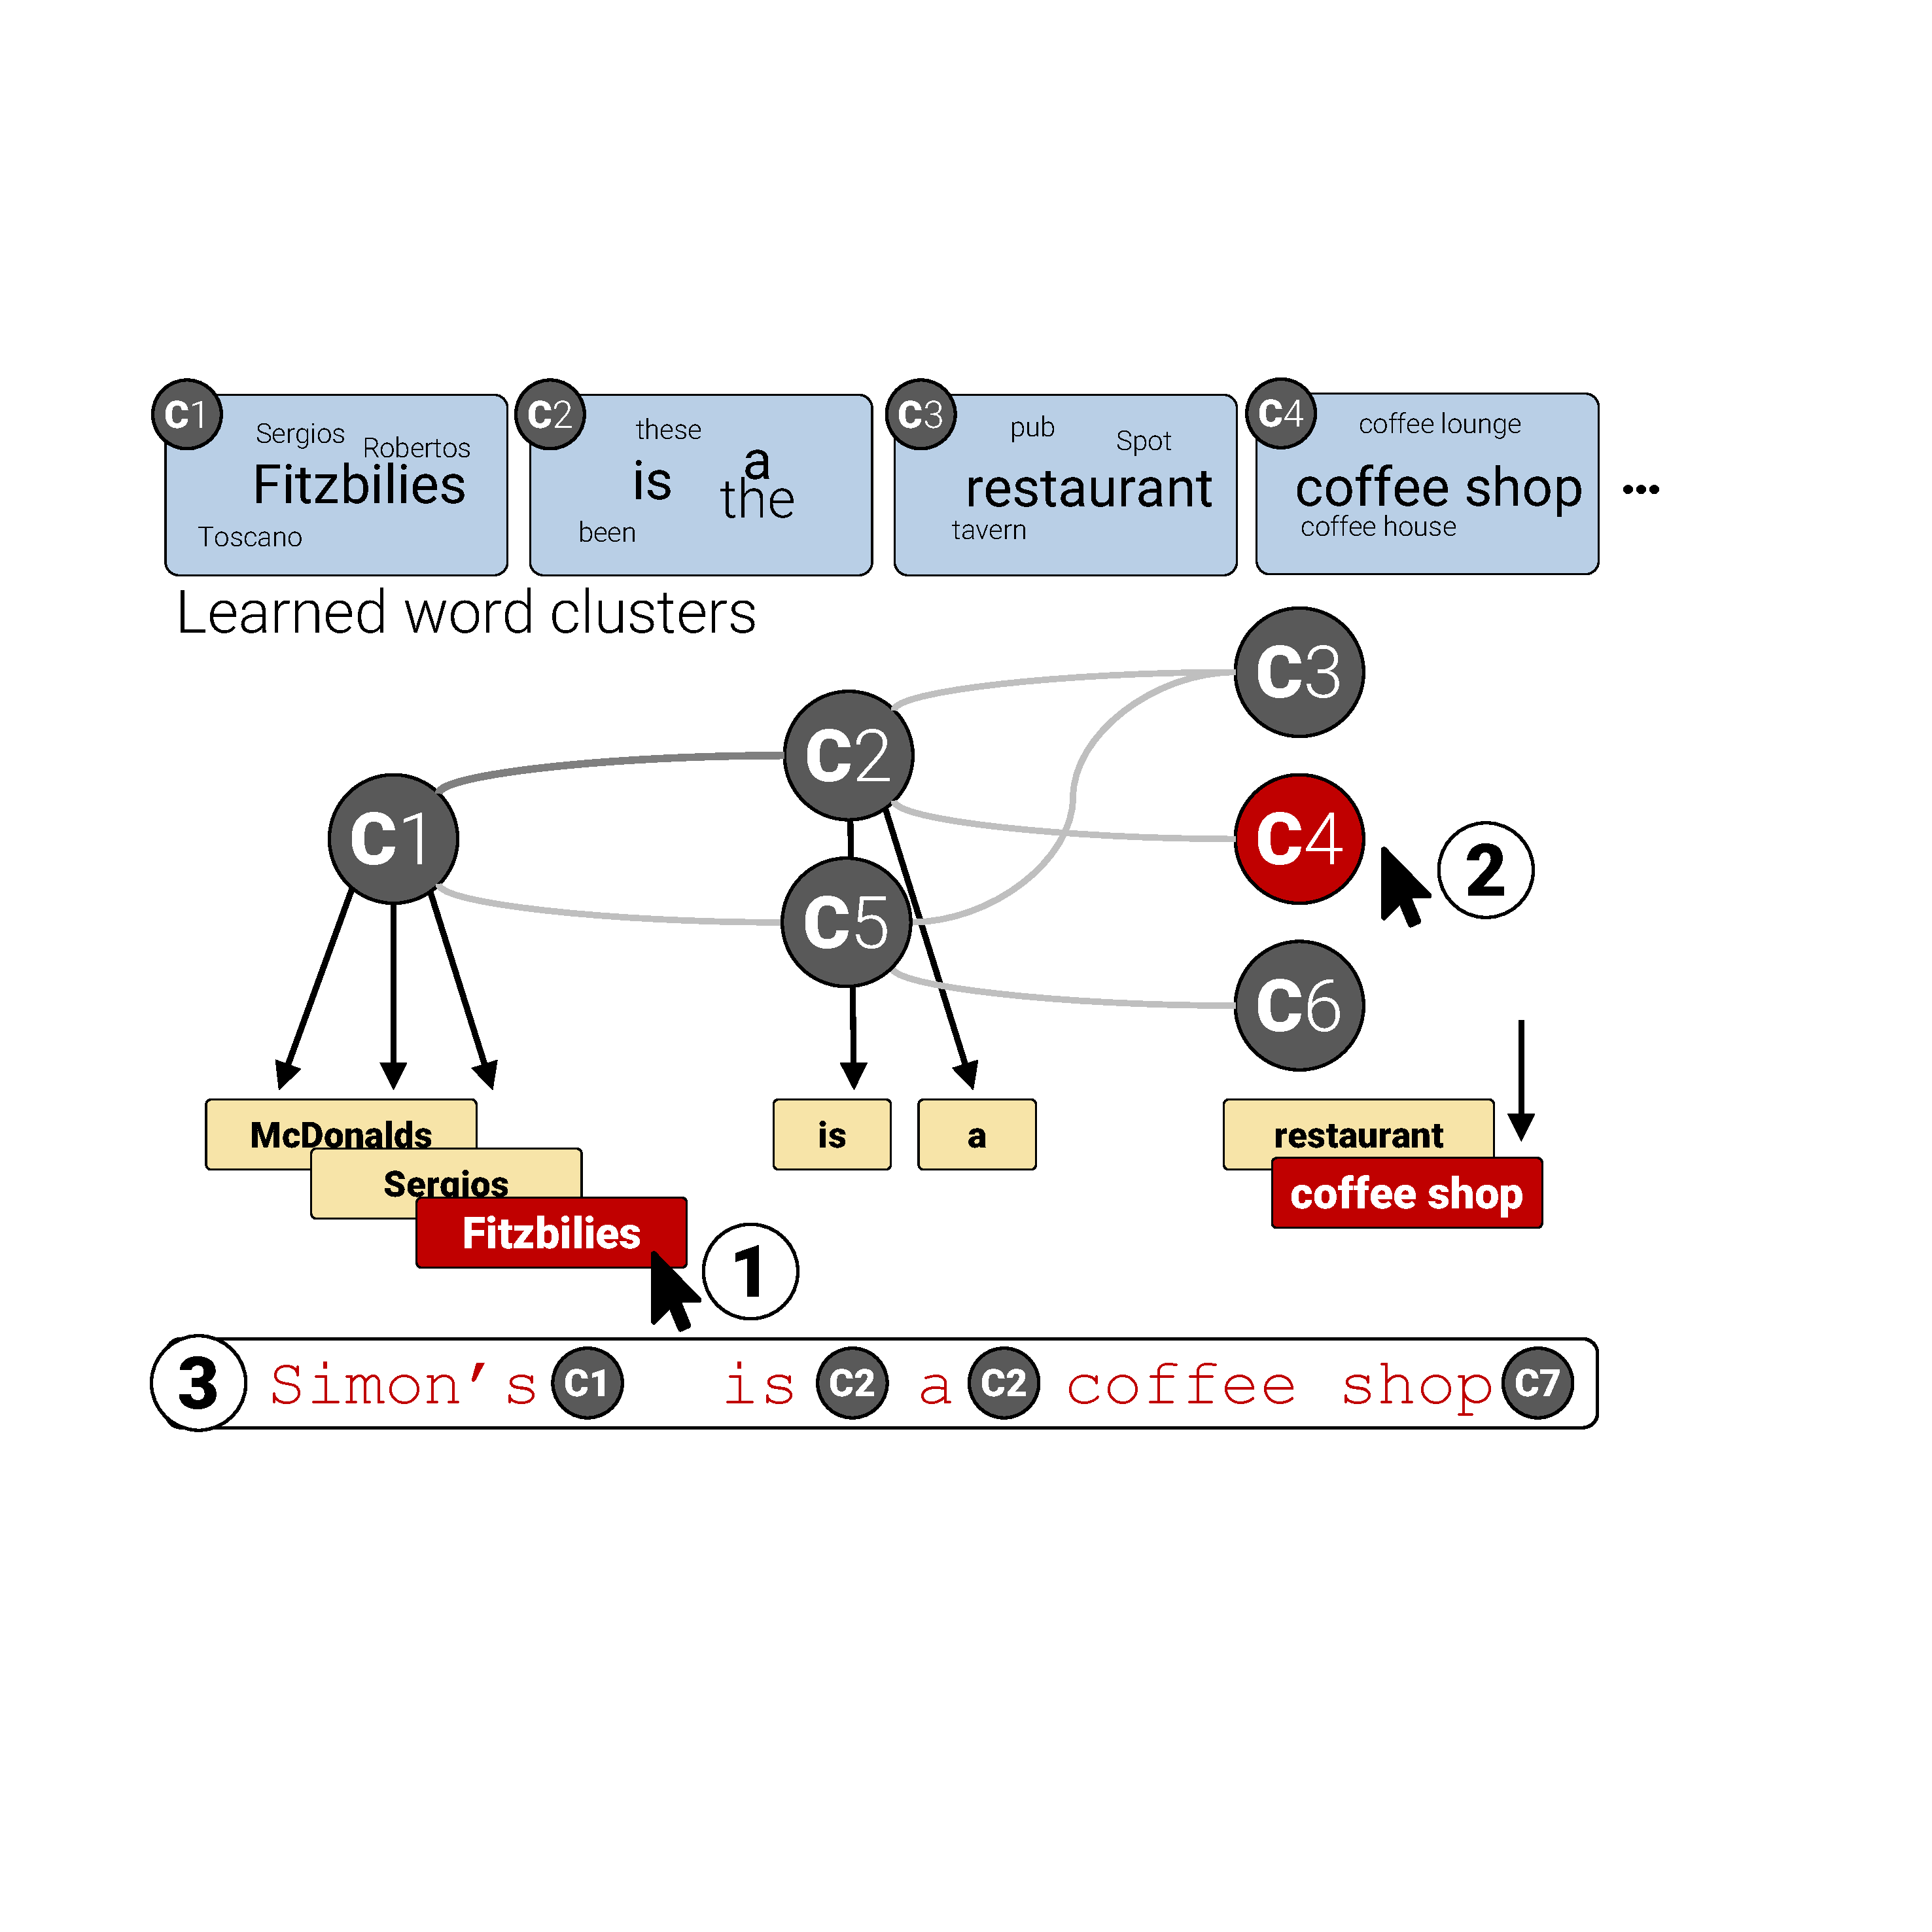
\includegraphics[width=0.7\textwidth]{DecoderVis}
  \end{center}
\end{frame}

\begin{frame}
  \begin{center}
    \textbf{(See Also) Latent Alignment and Variational Attention}


  \end{center}

  \begin{center}
    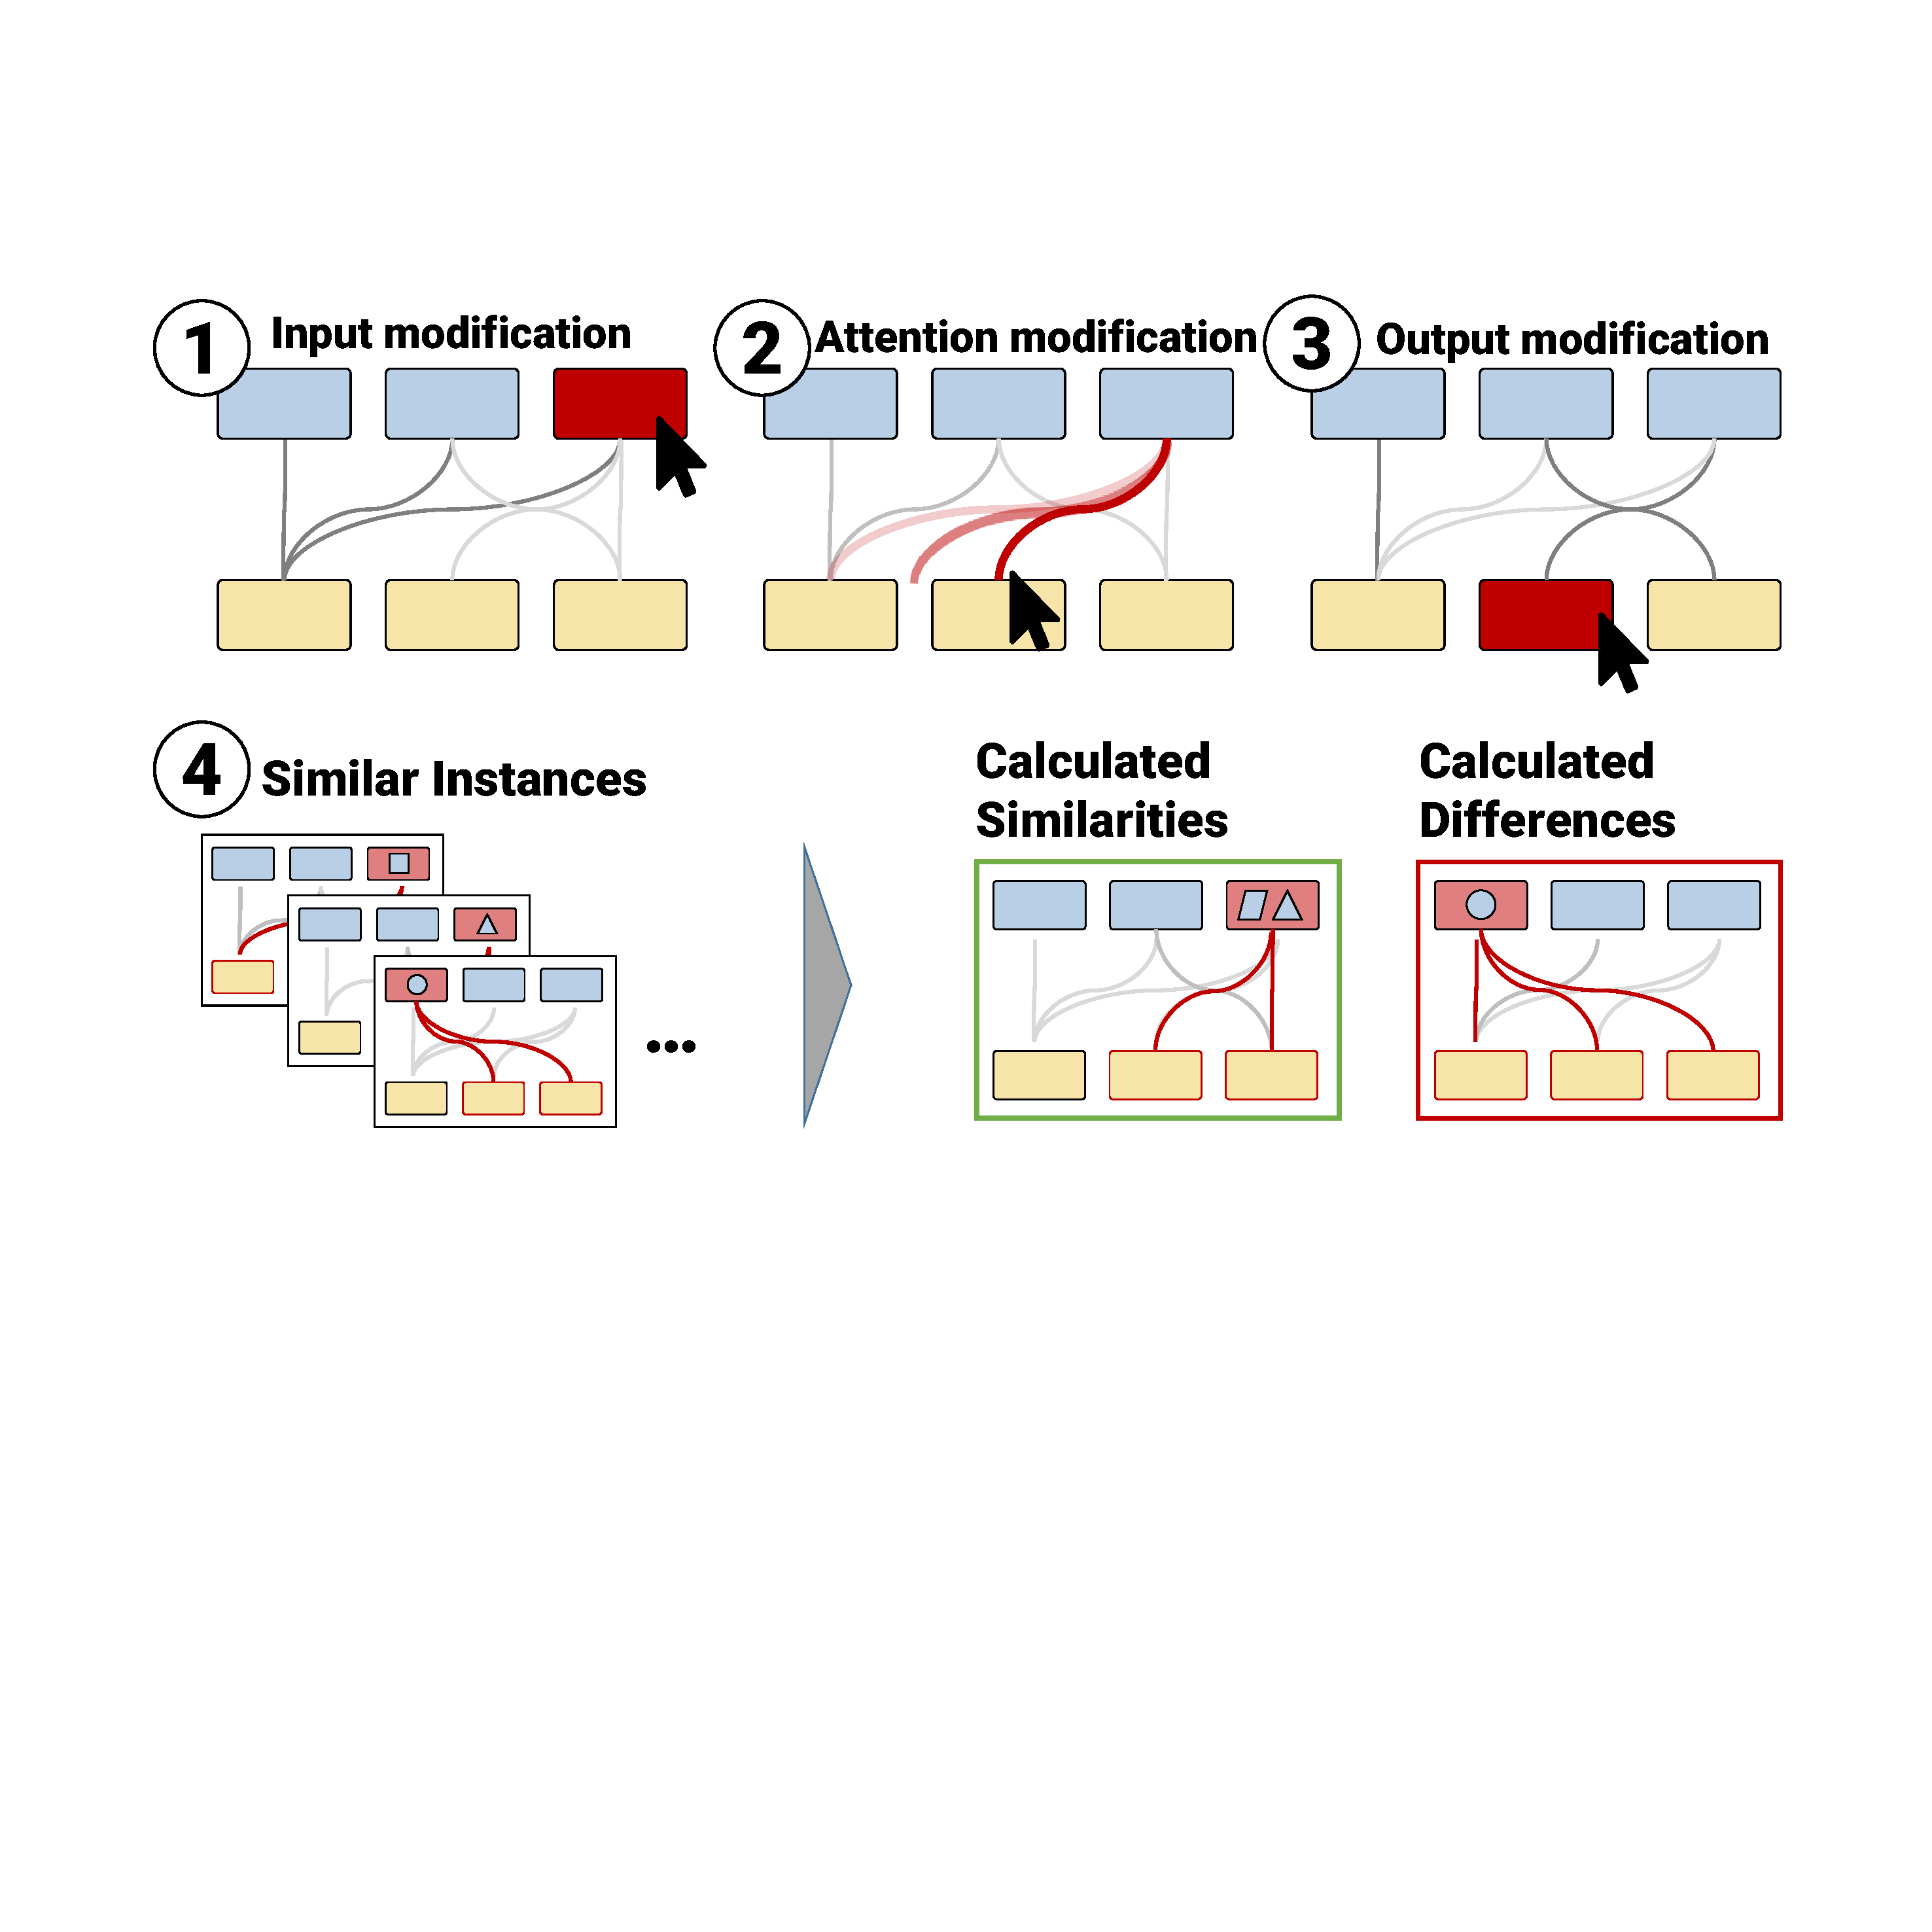
\includegraphics[width=0.7\textwidth]{AttentionVIS}
  \end{center}
\end{frame}

\section{Learning Neural Templates}




{
\setbeamercolor{background canvas}{bg=}
\includepdf[pages=2-2]{template}
\includepdf[pages=5-35]{template}
}

% \begin{frame}\thetitle{Method}
% \begin{figure}
%   \centering

%   \begin{tikzpicture}[every node/.style={anchor=base,minimum size=8mm}]
%     \matrix  (graph) [matrix of nodes, row sep=0.5em,column sep=-0.3em,
%     minimum width=0.2em, minimum height=0.5em, font=\small,ampersand replacement=\&] {
%       Mary \&
%       did \&
%       not \&
%       slap \&
%       the \&
%       green \&
%       witch \\
%       $z$ \& \& \& \& \& \& $\substack{\textcolor{blue}{p(z| x, \tilde{x})} \\ \textcolor{red}{q(z; x, \tilde{x}, y)} }$ \\
%       Maria \&
%       no \&
%       \textbf{daba} \&
%       una \&
%       bofetada \; a\&
%        la \; bruja \&
%       verde\\
%     };


%     \begin{scope}[on background layer]
%       \draw[blue!30, line width=0.1mm] (graph-1-1) -- (graph-3-3);
%       \draw[blue!30,line width=0.8mm] (graph-1-2) -- (graph-3-3);
%       \draw[blue!30,line width=0.4mm] (graph-1-3) -- (graph-3-3);
%       \draw[blue!30,line width=0.6mm] (graph-1-4) -- (graph-3-3);
%       \draw[blue!30,line width=0.04mm] (graph-1-5) -- (graph-3-3);
%       \draw[blue!30,line width=0.5mm] (graph-1-6) -- (graph-3-3);
%       \draw[blue!30,line width=0.15mm] (graph-1-7) -- (graph-3-3);

%       \draw[draw=red!30, line width=0.2mm] ($(graph-1-1) + (0.1, 0)$) -- ($(graph-3-3) + (0.1, 0)$);
%       \draw[draw=red!30, line width=0.2mm] ($(graph-1-2) + (0.1, 0)$) -- ($(graph-3-3) + (0.1, 0)$);
%       \draw[draw=red!30, line width=0.1mm] ($(graph-1-3) + (0.1, 0)$) -- ($(graph-3-3) + (0.1, 0)$);
%       \draw[draw=red!30, line width=0.9mm] ($(graph-1-4) + (0.1, 0)$) -- ($(graph-3-3) + (0.1, 0)$);
%       \draw[draw=red!30, line width=0.1mm] ($(graph-1-5) + (0.1, 0)$) -- ($(graph-3-3) + (0.1, 0)$);
%       \draw[draw=red!30, line width=0.4mm] ($(graph-1-6) + (0.1, 0)$) -- ($(graph-3-3) + (0.1, 0)$);
%       \draw[draw=red!30, line width=0.1mm] ($(graph-1-7) + (0.1, 0)$) -- ($(graph-3-3) + (0.1, 0)$);


%       \draw[rounded corners,fill=red!10] ($ (graph-3-1.north west) +(-0.1,0.1)$) rectangle  node[yshift=-0.8cm]{\textcolor{red}{}} ($(graph-3-7.south east) +(0.1,-0.1)$ ) ;

%       \draw[rounded corners,fill=red!10] ($ (graph-1-1.north west) +(-0.1,0.1)$) rectangle  node[yshift=0.8cm]{\textcolor{red}{}} ($(graph-1-7.south east) +(0.1,-0.1)$ ) ;

%       \draw[rounded corners,fill=green!10] (graph-1-1.north west) rectangle  node[ yshift =0.7cm] {$x_{1:T}$} (graph-1-7.south east);

%       \path[] (graph-3-3.north west) rectangle  node[yshift=-0.9cm]{\textbf{$y_3$}} (graph-3-3.south east);

%       \draw[rounded corners, fill=blue!10] (graph-3-1.north west) rectangle  node[yshift=-0.9cm]{\textcolor{blue}{$\tilde{x}$}}  ($(graph-3-2.south east) + (-0.1, 0)$);

%     \end{scope}
%   \end{tikzpicture}


%   A sketch of variational attention applied to translation.
%   \begin{itemize}
%   \item  The blue prior $p$ is restricted to past information,
%   \item  The red variational posterior $q$ may take into account future observations.
%   \end{itemize}
% \end{figure}
% \end{frame}


\begin{frame}
  \thetitle{Interpretability and Robustness in Generation}

  \begin{itemize}
  \item End-to-end modeling gives accurate and natural responses.
    \air

  \item Discrete structure provides high-precision guarantees.
    \air

  \item System is post-hoc checkable and adjustable by humans.

  \end{itemize}

\end{frame}


\section{Conclusion}

\begin{frame}
  \thetitle{Conclusion}
  \begin{itemize}
  \item Discrete latent variables are a natural fit for NLP
    \air
  \item Methods can be integrated naturally into many problems.
    \air
  \item Tools for training these approaches are coming along fast. (Pyro, Edward, etc.)
    \air

  \item Also check out our tutorial: Deep Latent-Variable NLP
    \url{bit.do/lvnlp}

  \end{itemize}
\end{frame}

\end{document}
